\setlength\paperheight{11in}
\setlength\paperwidth{8.5in}

\documentclass[9pt,twocolumn]{article}
\usepackage[9pt,inchmargins,nocopyright]{sigmin}
\usepackage{color,url,graphicx,hyperref,tabularx,colortbl}
\usepackage{microtype,times,multirow,amsthm,xspace}
\usepackage[square,comma,numbers,sort&compress]{natbib}
\usepackage{float}
\usepackage{framed}
\usepackage{mathptmx}

% \clubpenalty=10000
% \widowpenalty=10000

\setlength\pdfpageheight{\paperheight}
\setlength\pdfpagewidth{\paperwidth}

\hyphenation{App-Engine php-BB}
\renewcommand{\ttdefault}{pxtt}
\newcommand{\name}{CryptDB\@\xspace}

\begin{document}

\title{\bf CryptDB: Protecting Confidentiality with \\
	   Encrypted Query Processing}
\author{Raluca Ada Popa, Catherine M. S. Redfield,
	Nickolai Zeldovich, and Hari Balakrishnan \\
	MIT CSAIL}
\date{}

\newcommand{\RND}{\textrm{RND}}
\newcommand{\DET}{\textrm{DET}}
\newcommand{\OPE}{\textrm{OPE}}
\newcommand{\OPEJOIN}{\textrm{OPE-JOIN}}
\newcommand{\HOM}{\textrm{HOM}}
\newcommand{\JOIN}{\textrm{JOIN}}
\newcommand{\SEARCH}{\textrm{SEARCH}}

\newcommand{\up}{\texttt{UPDATE}}
\newcommand{\ins}{\texttt{INSERT}}
\newcommand{\del}{\texttt{DELETE}}
\newcommand{\sel}{\texttt{SELECT}}

\newcommand{\rap}[1]{\textcolor{blue}{RAP: #1}}
\newcommand{\hb}[1]{\textcolor{red}{HB: #1}}
\newcommand{\nz}[1]{\textcolor{magenta}{NZ: #1}}
\newcommand{\cmsr}[1]{\textcolor{green}{CR: #1}}
\newcommand{\todo}[1]{\textcolor{red}{#1}}


\newcommand{\tput}{27\%}

\newtheorem{definition}{Definition}
\newtheorem{theorem}{Theorem}

\maketitle

% !TEX root = paper.tex

\begin{abstract}

  Online applications are vulnerable to the theft of sensitive
  information because adversaries can exploit software bugs to gain
  access to private data, and because curious or malicious
  administrators may capture and leak data.  \name is a system that
  provides practical and provable confidentiality in the face of these
  attacks for applications backed by SQL databases.  It works by fully
  {\em executing SQL queries over encrypted data} using a collection of
  efficient SQL-aware encryption schemes.  \name also {\em
    chains encryption keys to user passwords}, so that a data item can
  be decrypted only using the password of one of the users with access
  to that data.  As a result, even if the adversary compromises all servers,
  he or she cannot decrypt the data of any user that is not logged in.
  Our evaluation shows that \name has low overhead: on a real application, phpBB, \name{} reduces throughput by 
  13\%, and on the TPC-C
  benchmark by 27\% compared to regular
  Postgres.  Chaining encryption keys to user passwords requires
  11--13 unique schema annotations for database schemas of three
  multi-user web applications to capture their policies.

  % Encrypting each user's data with different keys requires XXX lines of
  % annotations in phpBB (a popular web bulletin board) and XXX lines of
  % annotations in the HotCRP conference review system.

%   Importantly, \name does not change the innards of existing DBMSs:
%   we realized the implementation of \name using client-side query
%   rewriting/encrypting, user-defined functions, and server-side tables
%   for public key information. As such, \name is portable; porting
%   \name to MySQL required changing 86 lines of code, mostly at the
%   connectivity layer.

\end{abstract}

% !TEX root = paper.tex

\section{Introduction}
\label{s:intro}

\begin{figure*}
\centering
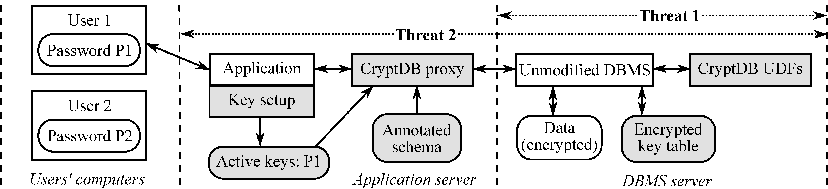
\includegraphics{fig/overview}
\caption{\name's architecture, made up of two parts: a {\em database
    proxy} and an unmodified {\em DBMS}, which uses
  user-defined functions (UDFs) to implement components of \name{}.
  Rectangular and rounded boxes represent processes and data,
  respectively.  Shading indicates components added by \name.  Dashed
  lines indicate separation between users' computers, the application
  server, and the DBMS server.  \name{} addresses two kinds of
  threats, shown as dotted lines.  In threat 1, a curious database
  administrator with complete access to the DBMS server snoops on
  private data, in which case \name{} leaks no data.  In threat 2, an
  adversary gains {\em complete} control over both the software and
  hardware of the application and DBMS servers, in which case
  \name{} leaks no data of currently inactive (not logged in) users
  (data of user 1 in this example may leak).}

\label{fig:overview}
\end{figure*}

% \nz{Today: no privacy guarantees if application/server/database are
% compromised.  This paper is about how to provide some privacy guarantees
% in the face of arbitrary server compromises.  Need to compare briefly
% to apps that either don't trust the server (SPORC, Depot), or that
% don't need a server: Ivy~\cite{muthitacharoen:ivy}, peer-to-peer apps:
% not all apps can be distributed across clients, and even when possible,
% it's difficult to do for existing server-side applications.}

Theft of private information is a significant problem, particularly
for online applications~\cite{prc:breaches}.  An adversary can exploit
software vulnerabilities~\cite{cve:stats} and bugs to
gain unauthorized access to servers; curious or malicious
administrators at a hosting or application provider can snoop on
private data~\cite{chen:gmail-snooping}; and attackers with
physical access to servers can cause significant
damage~\cite{halderman:cold-boot}.

%Although an impressive amount of work has gone
%into preventing compromises in the first place, vulnerabilities and
%attacks remain commonplace~\cite{prc:breaches,cve:stats}.

One approach to reduce the damage caused by server compromises is to
encrypt sensitive data, as in SUNDR~\cite{li:sundr},
SPORC~\cite{feldman:sporc}, and Depot~\cite{mahajan:depot}, and run
all computations (application logic) on clients.  Unfortunately,
several important applications don't lend themselves to this approach,
such as a database-backed web site that processes queries to generate
data for the user, or an application that computes over large amounts of data.  Even when this approach is
tenable, converting an existing server-side application to this form can be
difficult.  On the other hand, one might consider theoretical solutions such as fully-homomorphic
encryption~\cite{gentry:fhe} to allow servers to compute over
encrypted data.  However, these schemes are currently wildly
impractical, with slowdown estimates on the order of a trillion
times~\cite{trillion}.

This paper presents \name{}, a system that explores an intermediate
design point to provide practical privacy guarantees for applications
that use database management systems (DBMSs).  \name leverages the
typical structure of database-backed applications, consisting of a
DBMS server and a separate application server, as shown in
Figure~\ref{fig:overview}; the latter runs the application code and
issues DBMS queries on behalf of different users.  \name's main idea
 is to {\em execute queries over encrypted data} and the key insight
that makes it practical is that SQL uses a well-defined set of
operators, each of which we are able to run over
encrypted data.

\name{} addresses two threats.  The first threat is a {\em curious
  database administrator} (DBA) who tries to learn private data (e.g.,
health records, financial statements, personal information, etc.) by
snooping on the DBMS server; here, \name ensures that the DBA cannot
extract any private data.  The second threat is an {\em adversary that
  gains complete control of application and DBMS servers}.  In this
case, \name cannot provide any guarantees for users that are logged-in the application during an attack, but still guarantees the confidentiality of
other users' data.

% In this paper, we consider a design point between ``no server
% computation'' and ``arbitrary server computation'': {\em perform SQL
% query execution over encrypted data}.  SQL relational databases are
% widely used and perform non-trivial (though not entirely arbitrary)
% computations.

% We present {\em \name{}}, a practical system that executes SQL queries
% and transactions over encrypted data without decrypting the data to a
% clear-text format, providing strong privacy guarantees in the face of
% server compromises.  With \name{}, the DB server is entirely
% untrusted, and application servers are trusted only with respect to
% the private data of principals---e.g., web application users---who are
% currently logged in.

% Database management systems (DBMSs) are
% an especially appealing target for attackers, because they often
% contain large amounts of private information.  When individual
% users or enterprises store their sensitive data in a DBMS today, they
% must trust that the server hardware and software are uncompromisable,
% that the data center itself is physically protected, and assume that
% the system and database administrators (DBAs) 
% %who maintain the DBMS software 
% are trustworthy.  Otherwise, an adversary who gains access to any of
% these avenues of attack can compromise the entire database, as has
% been documented in a number of published reports of data
% thefts~\cite{prc:breaches} (and presumably there are more
% compromises that have not been publicized).

% These stringent security requirements are also at odds with
% cost-saving measures such as the consolidation of DBMSs belonging to
% different business units into a common enterprise-wide IT
% infrastructure, moving databases into a public cloud, or outsourcing
% DBA tasks.  In fact, ``lack of trust'' is an oft-quoted primary
% concern about moving data in database systems to more cost-effective
% cloud infrastructures.  Moreover, thanks to high-profile thefts of
% social security identifiers, credit card numbers, and other personal
% information from various online databases, these concerns are
% increasingly being reflected in the law as well: for instance, recent
% legislation requires that all databases containing personal data about
% Massachusetts residents be encrypted~\cite{Masslaw}.



% A significant barrier to deploying database systems in the cloud is
% the perceived lack of privacy, which in turn reduces the degree of
% trust users are willing to place in such deployments. If clients were to
% encrypt all the data stored in the cloud database, and if the data
% were decrypted only on client-controlled machines, then privacy
% concerns would largely be eliminated. Similarly, even in so-called
% private clouds inside enterprises, users often desire the ability to
% store data and run queries in data centers without trusting the
% database and system administrators with the content.

%In \name, unmodified DBMS servers store {\em all} sensitive data in
%an encrypted format, and execute SQL queries over encrypted data without
%having access to the decryption keys.  

% \hb{May not be necessary for SIGMOD.}
% SQL provides a good trade-off between generality and efficiency in cloud storage.
% On the one hand, SQL is widely used and useful to the many applications that
% already store their data in SQL databases, and use SQL queries to efficiently
% process their data.  On the other hand, SQL provides a structured data
% representation and a declarative query language that is much easier to reason
% about and to process efficiently over encrypted data than a general-purpose
% computation.


% \hb{Less related work here.}
% While early proposals attempted to enable SQL processing over encrypted
% data~\cite{sqlOverEncryption}, their privacy mechanisms were mostly heuristic,
% required a significant rewrite of the DBMS design, relied on considerable
% client-side processing, and did not support certain SQL queries. More recent
% literature~\cite{Dawn-Song-Search-2000, Chang04privacypreserving,
% queriesEncryptionBoneh,
% amanatidis-boldyreva-o'neill, Yang-privacy-preserving-queries,
% encrypt-for-secure-outsource, private-query-multi-user-for-searchable} has
% developed cryptographic tools for searching keywords on encrypted data and has
% proposed using these tools to process SQL queries on encrypted data. Although such
% work is a good first cut at the problem, it does not provide a
% comprehensive systems solution: they do not support many basic SQL queries (and
% mostly only support equality comparisons), some of them require significant
% client-side query processing, change the internal processing of a DBMS, and many
% of these schemes are too inefficient (requiring users either to build and maintain
% indexes or to perform sequential scans for every selection).

There are two challenges in combating these threats.  The first lies
in minimizing the amount of data revealed to the DBMS server, without
sacrificing the ability to execute queries efficiently.  Using
a single key to encrypt each row in the database would not allow the
DBMS server to execute many SQL queries without access to the
decryption key; consider, for instance, a query that asks for the
average salary of employees or for the names of employees whose salary
is greater than \$60,000.  These queries require computing over
encrypted data, but existing approaches that provide this capability
are either too slow for real-world use or don't provide adequate
confidentiality.  An ideal solution should impose a low performance
overhead on the DBMS server, avoid executing queries outside the DBMS,
and run on unmodified DBMS server software to benefit from decades of
engineering effort in optimizing DBMS performance.

%Moreover, a practical solution would operate not
%require DBMS software changes, to take advantage of decades of
%engineering and optimization work.

The second challenge is to minimize the amount of data leaked when an
adversary compromises the application server.  An ideal solution would
ensure that the application can issue queries only for data it
legitimately requires, and not for arbitrary data requested by an
adversary.  However, this task is difficult because the DBMS server
can also be subverted by the attacker, so \name cannot trust it to
prevent the application from reading arbitrary data.  Moreover, the
application itself has legitimate access to \name{}'s decryption keys,
and assigning each user a different database encryption key is
inadequate for applications with shared data, such as a bulletin board
or a conference review site.

%that gains access to the database and application servers can subvert
%both of them.

% \nz{Do we really need this challenge?}  \hb{I think we should rewrite
%   this challenge somehow to get at the adjustable encryption solution:
%   i.e., somehow say that there might be the equivalent of ``the
%   minimum required information'' to process a query and we want to get
%   that.}  

% The third challenge is in designing a system that balances the need
% for server-side computation with the need to minimize information
% revealed to the untrusted DB server.  An ideal solution would reveal
% only the smallest amount of information about the data required to run
% any given query mix.

% The third challenge is to carefully define ``privacy'' for
% an untrusted DBMS, as well as come up with a system design that
% provably achieves that definition.  On the one hand, even if all of
% the data stored on a DBMS server were encrypted, the server must be
% able to perform certain operations on the rows, such as aggregations,
% selections, and joins.  On the other hand, an adversary that
% compromises a DBMS server may now learn information about the data,
% such as relations between different rows in a table.  Thus, we need to
% define privacy in a way that balances the need for server-side
% computation with the need to minimize information revealed to the
% server.

\name{} addresses these challenges using three novel ideas.  The first
is to {\em execute SQL queries over encrypted data}.  \name{}
implements this idea using an {\em SQL-aware encryption strategy},
which leverages the fact that all SQL queries are made up of a
well-defined set of primitive operators, such as equality checks,
order comparisons, aggregates (sums), and joins.  By adapting known
encryption schemes (for numeric and string equality, additions, and
order checks) and using a new privacy-preserving cryptographic method
for joins, \name{} encrypts each data item in a way that allows the
DBMS to execute on the transformed data.
%For example, to perform
%equality checks over encrypted data, \name encrypts data with a
%deterministic encryption scheme, so that equal plaintexts have equal
%ciphertexts.  
\name{} is efficient because it mostly uses symmetric-key encryption,
avoids fully-homomorphic encryption, and runs on unmodified DBMS
software (with user-defined functions).

Some encryption schemes leak more information about the data to the
DBMS server than others, but are required to process certain queries.
To avoid revealing all possible encryptions of data to the DBMS {\em a
  priori}, \name carefully {\em adjusts} the SQL-aware encryption
scheme for any given data item, depending on the queries observed at
run-time.  To implement these adjustments efficiently, \name{} uses
{\em onions of encryption}.  Onions are a novel way to compactly store
multiple ciphertexts within each other in the database and avoid
expensive re-encryptions. % in the proxy.

% The second technique is {\em adjustable query-based
%   encryption}, where \name chooses the most secure encryption scheme
% that still allows queries to execute, based on the queries at runtime.
% Finally, \name uses a third technique, {\em onions of encryption}, to
% compactly store multiple ciphertexts in the database, and to adjust
% encryption schemes without re-encryption in the proxy.


% because the bulk of the DBMS, including query planning, data layout,
% transaction coordination, and the structure of the queries themselves,
% remain unchanged.

% The third idea is {\em adjustable query-based encryption}, where
% \name{} dynamically adjusts the encryption level for each data item at
% run-time, to achieve the maximum privacy level given the query mix.
% The \name{} frontend initially encrypts all data with the strongest
% level of encryption; as the application issues SQL queries, it adjusts
% the level of encryption on the server, so that the server can perform
% the classes of computations necessary for that SQL query.  \name{}
% implements adjustable query-based encryption by encrypting each data
% item in an {\em onion of encryptions}, from weaker forms of encryption
% that allow certain computations, to stronger forms of encryption that
% reveal no information, as shown in Figure~\ref{fig:onion}.  This
% approach allows the frontend to efficiently adjust encryption levels
% on the server without having to re-encrypt all data at the client.

%the same, and only individual SQL operators used by a query may need
%to change.

% \hb{Walfish found this para confusing...}  

The third idea is to {\em chain encryption keys to user passwords}, so
that each data item can only be decrypted through a chain of keys
rooted in the password of one of the users with access to that data.
As a result, if the user is not logged into the application, and if
the adversary does not know the user's password, the adversary cannot
decrypt the user's data, even if the DBMS and the application server
are compromised.  To construct a chain of keys that captures the
application's data privacy and sharing policy, \name allows the
developer to provide policy annotations over the application's SQL
schema, specifying which users (or other principals, such as groups)
have access to each data item.

%Programmers use annotations to specify application-level
%principals, such as users in a web application, and the data that each
%principal should have access to, 

%\name{} also uses a novel SQL
%schema annotation language that allows programmers enforce individual
%users' privacy at the level of SQL queries, with minimal changes to
%their application.

% For
% example, the outermost layer uses randomized encryption, which
% guarantees that the server can learn nothing about the data, aside
% from its length.  If the user issues an SQL query containing {\tt
%   WHERE id=5}, \name{} sends the server an {\em onion key} to decrypt
% the {\tt id} column to a deterministic encryption level, where
% identical plaintexts have identical ciphertexts.\footnote{\name
%   never gives the server onion keys to decrypt the data to plaintext.}
% \name{} then sends the server a deterministic encryption of the
% constant 5, allowing it to compute matching rows by only revealing
% the necessary {\em relations between data items}, and {\em not
%   revealing the actual data}, or other relations between data items
% not used in this query.


% Privacy and practicality are 
% conflicting goals. At one extreme, theoretical approaches using fully homomorphic
% encryption~\cite{gentryVerifiable} support any general computation
%  on encrypted data and provide strong privacy guarantees (e.g., the DBMS
% does not even learn access patterns). Unfortunately,
% such approaches are prohibitively impractical; for example, performing a simple
% string search using homomorphic encryption is about a trillion times slower than without
% encryption~\cite{trillion}. At the other extreme, providing no privacy by
% keeping the data in the clear, provides high performance and functionality.

% The idea for achieving practical privacy is \textit{to
% allow the database server to process queries on encrypted data as it would do on clear
% data}; when the server needs to evaluate a predicate on two encrypted data
% items, we empower the server to do so.

% In this model, each query requires the server to perform a certain class of
% computations on stored data. For example,
% consider evaluating an equality filter such as \texttt{WHERE id = 5}. Given
% the encryption of 5, say \texttt{x1c5a21}, the server needs to be able to
% figure out what rows in column \texttt{id} have an encryption of
% \texttt{x1c5a21}.  \name{} allows the server to compute the set of rows whose
% {\tt id} column matches the given ciphertext, but does not reveal to the
% server the original values, or what plaintext \texttt{x1c5a21} corresponds to.
% That is, \name{} reveals the {\em relations between data} that the server needs
% to know to execute a type of query, but {\em not the actual data}, or any
% relations over encrypted data not queried by the user.

% As such, \name{} provides maximum privacy given the classes of computations
% required for the user's queries.
% To the best of our knowledge, \name{} provides stronger privacy guarantees than
% any previous work that is practical and as functional. \name{} ensures that
% the database server only stores and
% manipulates encrypted data. By encrypting all data stored on the database server,
% the solution prevents the database administrator (DBA) from extracting private
% data, while still being able to manage and tune the database server.

% To enable the server to perform user-requested queries, we build on existing
% cryptographic tools, optimize others, as well as design a new
% cryptographic primitive. For example, any deterministic encryption scheme
% (denoted $\DET$) allows equality checks because
% the same value will be mapped to the same ciphertext. Any encryption scheme that
% preserves the order of the values encrypted (denoted $\OPE$) allows range
% queries. For joins, we design a new cryptographic primitive that enables the
% server to join only the columns requested by the user.

% A natural question arises: without {\em a priori} knowledge of the queries to be
% performed, how can we know how to encrypt the data? Each data field must be
% encrypted according to the operations
% that will be performed on it. Some applications have a fixed set of queries that
% will issue to the server; however, for some applications the mix of queries may
% be unknown or the set of queries may change (e.g., when
% adding new features). Recall that one of our goals is to run applications on top
% of \name{} unchanged.

%\name{} works by rewriting SQL queries, storing encrypted data in
%regular tables, and using an SQL user-defined function (UDF) to
%perform server-side cryptographic operations.
 
 
 % OUR SUMMARY
%Results show that \name incurs a throughput overhead of
%13\% for phpBB and 27\% for TPC-C which we consider acceptable considering the added confidentiality, requires 11--13 lines of unique annotations to secure more than twice,  and supports all queries on TPC-C and  on three applications. and app functionality

We have implemented \name{} in a way that should work with most
standard SQL DBMSes, and ran it on both unmodified Postgres and MySQL
servers. We ran \name{} on three multi-user web applications: phpBB (a
popular online bulletin board), HotCRP~\cite{kohler:hotcrp}
(a conference review system),
and grad-apply (the graduate admissions system for MIT EECS), and on the
industry-standard TPC-C benchmark. \name{} secured all sensitive
fields in the three applications with only 11--13 unique
annotations, which expressed a variety of policies (including an
interesting new one in HotCRP for handling papers in conflict with a
PC chair).  \name{} supported all queries on encrypted data from these
applications.  Compared to an unencrypted DBMS, \name{} reduced
throughput by a modest 13\% for phpBB and 27\% for TPC-C\@.

%Porting \name{} to a new DBMS
%server is straightforward: our port to MySQL required changing just
%86 lines of code dealing with database connectivity and user-defined
%function specification. 
 

% In terms of development effort,
% \name{} requires XXX annotations for per-user encryption of private
% data in phpBB, a popular web bulletin board application, and incurs a
% throughput overhead of XXX.  \hb{HotCRP.}  \nz{grad-apply.}  


% In summary, this paper makes the following three contributions.
% First, we present the design and implementation of \name, a novel
% and practical system for protecting data privacy in an untrusted DBMS
% server by storing only encrypted data on the server running SQL
% queries without decrypting the data on the server.  Second, we
% introduce the idea of adjustable security, optimize existing
% cryptographic tools for use in SQL queries, and develop a novel
% cryptographic technique for privacy-preserving joins.  Third, we
% evaluate \name{} on a TPC-C workload \nz{and the database used by the
%   graduate admissions web site of our department, grad-apply, if we get
%   around to it}, and show that \name{} requires no application changes
% and imposes a modest 28\% throughput overhead.  Moreover, in addition
% to not requiring any modifications to DBMS server software, we show
% that porting \name{} entails only a modest amount of work: by changing
% just 85 lines of code (mostly connectivity code), we ported \name
% from Postgres to MySQL.

%\begin{CompactEnumerate}
%  \item The design of \name, a system that preserves privacy while allowing
%  SQL queries on encrypted data. \name:
%  \begin{list}{\labelitemi}{\leftmargin=1em}
%    \item provides provable guarantees of privacy (Sec. \ref{s:model}),
%    \item provides more
%    functionality than previous practical schemes by engineering existing 
%    cryptographic tools,
%    optimizing others, and designing a new cryptographic tool for
%    private joins,
%    \item does not require modification of client applications or prior knowledge of 
%    queries by the new mechanism of \textit{adjustable security} (Sec.
%    \ref{s:design}),
%    \item requires virtually no client side processing.    
%  \end{list}
%  \item The implementation and evaluation of \name{} on Postgres. \name:
%  \begin{list}{\labelitemi}{\leftmargin=1em}
%    \item does not change the DBMS so it can be ported to any standard
%    DBMS\@. By changing 85 lines of code of \name{} (mostly connection code
%    to the DBMS), we ported \name{} to MySQL (Sec. \ref{s:impl}),
%    \item has a modest overhead with a throughput loss
%    of $\approx 28\%$ on TPC-C (Sec. \ref{s:eval}).
%  \end{list}
%\end{CompactEnumerate}

% \hb{Not sure we need this para...}
% The rest of this paper is structured as follows.  First, \S\ref{s:model}
% describes \name's threat model.  \S\ref{s:design} presents \name's
% design in more detail, and \S\ref{s:impl} discusses our prototype
% implementation.  Our experimental results are presented in \S\ref{s:eval}.
% We compare \name{} to related work in \S\ref{s:related}, and conclude
% in \S\ref{s:concl}.





\section{Threat Model}
\label{s:model}

% As described in the previous section,
The goal of CryptDB is to ensure
the \textit{secrecy} of data in an SQL database in the face of \textit{an
adversary that has complete access to the database server}. The adversary could
compromise the server software, or even physically attack the server by stealing
and reading disks. Consequently, CryptDB makes \textit{no assumptions about the
database server keeping any data private}. This model covers all of the
motivating scenarios we have mentioned so far, such as outsourcing a SQL
database to the cloud, protecting against a curious database administrator,
and guarding against attackers breaking into the database server machine.
On the other hand, CryptDB assumes that the application and the CryptDB
frontend (Figure~\ref{fig:architecture}) are not compromised, and do not
reveal their keys to the adversary.  Dealing with attacks on these components,
such as SQL injection vulnerabilities or authentication bypass attacks, is
outside of the scope of this paper.

For the purposes of this paper, we assume that a malicious server does not
change the data or query results.  Ensuring integrity for SQL queries has
been heavily researched, and we refer to prior literature for techniques
to achieve integrity, as follows.  Since CryptDB allows the DBMS to process
relational queries on encrypted data as it would on plaintext data, most
previously-proposed approaches can be readily used with CryptDB\@.
A malicious server can affect three aspects of data security:
integrity, freshness, and completeness. Integrity is solved by adding
a MAC to each tuple as in~\cite{li:sundr,plutus,sirius}. Freshness
has been addressed using Merkle hashes or chained
hashes~\cite{plutus,cloudproof,sirius} and both freshness and
completeness of query results are addressed in~\cite{queryassurance}.
Also,~\cite{Li-Reyzin-06authenticatedindex}
and~\cite{Thompson_privacy-preservingcomputation} allow the client to verify
results of aggregation queries, \cite{authenticate-join} authenticates joins,
and~\cite{sion-assurance} provides query assurance for most read queries.

% Outside of the DBMS server, CryptDB assumes that the client frontend is fully
% trusted to keep its keys private. As we will see, the frontend does little
% work: it simply encrypts and anonymizes queries, but does not execute them.
% Hence, we believe this is a reasonable assumption, because a shared database
% server in the cloud is both a more compelling target for an attacker,
% and is more exposed than an individual (application) server.
% Moreover, keeping a server private is much easier than keeping the data of
% many database machines private.  Furthermore, for cases in which an enterprise
% hosts a frontend in their local cluster, and outsources their database to the
% cloud, access to the frontend may be considerably hard to achieve from outside
% of the enterprise as compared to gaining access to the cloud DBMS\@.

\subsection{Security Definition}\label{s:def}

\textbf{Intuition}. At a high level, CryptDB's definition of privacy says
that \name{} only reveals the relations between tuples needed by the server
to perform certain computations; in other words, CryptDB provides
\textit{maximum privacy given the classes of computations needed at the
server} to process SQL queries.  More specifically, the definition says
two things:
\vspace{-0.15cm}
\begin{itemize}
  \item If users request no relational predicate filtering 
on a column (i.e., they only request projections and computation),
nothing about the column content is leaked; if the user requests equality checks
on a column, we reveal which items repeat in that column;
if the user requests inequality checks on a column, we reveal the order
of the elements in the column.  We never reveal the actual data content.

\item The server cannot
process queries (that is, discover new data relations) different from the ones
requested by the user.
\end{itemize}
\vspace{-0.15cm}
This intuition suffices to grasp CryptDB's security model, so the
reader uninterested in formalism can proceed to the ``Implications''
part of this section below (and perhaps return to the formal definition
of security later).

\textbf{Definition.}
To formalize cryptographic definitions, often times one defines an
\textit{ideal world} using oracles and then proves that the proposed protocol
has as much privacy as the ideal world with respect to
polynomial-time adversaries. We will instead use the term \textit{ideal
system}.

What is the ideal system considering our goals? It is a system in
which the server only learns the data relations that it needs in order to perform
typical SQL processing for user queries, and nothing else. This is equivalent to
the server having access to \textit{no data content}, but only to an oracle that
is willing to answer questions about the relations between data items, restricted
only to questions needed to process requested queries.

Given a query $Q$, let $\fu(Q)$ be the classes of computations needed by
$Q_i$; that is, the relations between tuples that the server is allowed
to know to process
the query. For example, if $Q$ is \texttt{SELECT * FROM table1, table2 WHERE
table1.c1 = table2.c2}, then $\fu(Q)$ consists of questions of the form: ``is
the $i^\mathrm{th}$ item in c1 equal to the $j^\mathrm{th}$ item in c2''.
Obviously, the server
needs to know this information to process a join, but it does not need to know
the actual value of the two items. In the Appendix, we describe $\fu$ precisely.

\begin{definition}[Ideal System]\label{def:sec}
Let $Q_1 \ldots Q_t$ be the queries users requested up to time $t$. The
database at the server consists of each data item encrypted with the strongest
encryption scheme (random). Moreover, the
server has access to an oracle that only answers questions from $\fu(Q_1) \cup \ldots \cup \fu(Q_t)$.
\end{definition}

Obviously, in the Ideal System, the server can process SQL queries on encrypted
data because all the information it needs are the relations in $\fu(Q_1)
\cup \ldots \cup \fu(Q_t)$, by the definition of $\fu$. At the same time, such
server always has the database encrypted with the strongest encryption scheme
that leaks nothing.

We want the server in \name{} to learn as much information as the server in the
Ideal System and we show this property in \S\ref{s:analysis}.

\textbf{Implications.} While CryptDB does not reveal any data item, it does not
hide data access patterns.  For example, the database server can
monitor the frequency with which some data item is returned in a result set.
Masking such access patterns from the server would incur significant
overhead~\cite{pir-survey}, require virtually an
overwrite of the underlying DBMS, add considerable client-side
processing, and preclude server-side optimizations. 

CryptDB's database server can also check any predicates used to
execute past user-requested SQL queries, both at the time the query is executed,
and at any later time.  For example, if the application were to
issue the query {\tt SELECT * FROM table1 WHERE c1 = x2ad412}, the server
would be able to check rows for this predicate; however, this will be mostly
useless to the server because \texttt{x2ad412} is an
encrypted value and all that the server learns is the number of rows that match
this unknown constant.

Note that, when the server needs to evaluate a predicate $P$ (say,
\texttt{id = x245ab1?}), the server is allowed to perform the class
of equality check computations on column {\tt id} (albeit checking for
equality with an encrypted value) rather than just the computation of
checking for a specific value.  As such, the server can check
predicates of the form \texttt{c1 = *}, where $*$ is any ciphertext,
but whose corresponding value the server does not know.  Therefore,
what the server learns is the frequency of repeats of values only in
column \texttt{c1}.

We considered allowing the server to check equality only for the
specific constant given by the user, but cryptographic primitives supporting
equality checks in this way are very expensive. Moreover, doing so will not
bring much additional privacy. The reason is
that, typically, user queries end up performing selection on the same column for
a variety of different constants; after a few such queries, the privacy of this
seemingly-stronger scheme will converge to the privacy of our scheme.

\subsection{User-enforced Security}

% \nz{This is really more of a safeguard against bugs in applications that
%     issue queries they did not mean to..  The threat model / security
%     guarantees remain the same, so we could move this text to design or
%     implementation.}

In certain applications, it may be difficult for a programmer to find
all of the queries issued by the application, making it difficult
to reason about the precise privacy guarantees that CryptDB will
provide.  In this case, CryptDB allows the programmer to optionally
annotate the schema (in the frontend, as defined in the next section)
by specifying the lowest security level allowed for each column.
For example, the programmer may allow equality checks, but may not
want to reveal order within the column.  In this case, CryptDB will
not allow the server to perform inequality checks, and reject any
query that requires such computations.

% Specifically, the programmer can annotate each column $c$
% in the schema using operations $>, <, =$ and security levels \texttt{order},
% \texttt{repeats}, and \texttt{random} (or full privacy).  For example,
% \texttt{c > order} means that order of
% items in column $c$ should not be revealed, but repeats can be revealed. The
% frontend will make sure not to provide capabilities to the server for lowering
% privacy beyond the repeats point.
%If a programmer intends to
%allow the user application to make requests needing more functionality than
%he imposed as minimum in the schema, he needs to make adequate provisions for
% such queries to be processed client-side or somewhere else.


% !TEX root = paper.tex

\section{Queries over Encrypted Data}
\label{s:design}


This section describes how \name{} executes SQL queries over encrypted
data.  The threat model in this section is threat 1 from
\S\ref{ss:dbthreat}; the DBMS machines and administrators are not
trusted, but the application and the proxy are trusted.
%(The next section
%removes these trust assumptions.)

\name{} enables the DBMS server to execute SQL queries on encrypted
data almost as if it were executing the same queries on plaintext
data. Existing applications do not need to be changed because the
proxy exports the same SQL interface as the DBMS\@. The DBMS's query
plan for an encrypted query is the same as for the original query.
However, the operators comprising the query, such as selections,
projections, joins, aggregates, and orderings, are performed on
ciphertexts, and use modified operators in some cases.

The \name{} proxy stores a secret master key, $\mathit{MK}$, and the database
schema.  The DBMS server sees an anonymized schema, encrypted user
data, and some auxiliary tables used by \name{}.  \name{} also equips
the DB server with \name{}-specific UDFs that enable the server to
compute on ciphertexts for certain operations.

Processing a query in \name{} involves four steps:
\begin{CompactEnumerate}
\item The application issues a query, which the proxy intercepts and
  rewrites: it anonymizes each table and column name, and, using the
  master key $\mathit{MK}$, encrypts each constant in the query with an
  encryption scheme best suited for the desired operation
  (\S\ref{ss:sqlaware}).
\item The proxy passes the query to its {\em onion key manager (OKM)}
  module, which assesses if the server should be given onion keys to
  execute the query. If so, the OKM does so by issuing an
  \texttt{UPDATE} query at the server that invokes a UDF to adjust the
  privacy level of the appropriate columns (\S\ref{ss:onion}).
\item The proxy forwards the encrypted query to the DBMS server,
  which executes it using standard SQL (occasionally invoking 
  UDFs for aggregation).
\item The DBMS server returns the query result, which the proxy
  decrypts and returns to the application.
\end{CompactEnumerate}

%To execute each SQL query, the proxy anonymizes, encrypts and rewrites
%the query before forwarding it to the untrusted DBMS server.  
% To anonymize a query, the proxy replaces each table with the table
% name from the anonymized schema (see Figure \ref{fig:schema}).  
% For
% projection, the proxy replaces each column with the name of the
% anonymized column for the first onion.  

\subsection{SQL-aware Encryption}
\label{ss:sqlaware}

The key idea to our design is that different encryption schemes enable
different SQL operations.  We use existing encryption schemes, optimize
a recent scheme, and design a new cryptographic primitive for joins.

\name{} uses the same key (derived from $\mathit{MK}$) to encrypt each  data item in a column so that the same computation can be performed on every
element in that column. (We will
  use finer-grained encryption in \S\ref{s:multi} to reduce the
  potential damage of application compromise.)

For each encryption type we use, we explain the security property that
\name{} requires from it, its functionality, and how to implement it with existing schemes. 
 
\textbf{Random} ($\RND$)\@. $\RND$ provides maximum security:
indistinguishability under an adaptive chosen-ciphertext attack
(IND-CCA2).  Two equal values will be
mapped to different encryptions with high probability. $\RND$ does not
allow any computation to be performed efficiently on the ciphertext.
To implement $\RND$, \name{} uses AES in UFE mode~\cite{desai:ufe}.

\textbf{Deterministic} ($\DET$)\@. $\DET$ has a slightly weaker
guarantee, yet is still has strong security: it only leaks which encrypted values correspond to the same
data value. This encryption level allows the server to perform
equality checks, which means it can perform selects with equality
filters, equality joins, {\tt GROUP BY}, {\tt COUNT}, {\tt DISTINCT},
etc.  There are
many ways to implement $\DET$, such as $\DET_K(v)=\RND_{K_1}(v) ~ \| ~
\textrm{HMAC-SHA1}_{K_2}(v)$, where $\|$ is the
concatenation operator, $K_1$ and $K_2$ are two keys derived from $K$,
and $K$ itself is derived by encrypting the table and column names
with $\mathit{MK}$\@.  For this $\DET$ construction, the server compares two
encryptions by comparing their HMAC-SHA1
values.
% We implement $\DET$ using AES in counter mode with a
% separate IV (counter value) for each column, derived by encrypting the table
% and column names with $\MK$\@.

\textbf{Order-preserving encryption} ($\OPE$)\@. $\OPE$ allows order
relations between data items to be established based on their
encrypted values, but does not leak any other information about the
data. If $x < y$, then $\OPE_K(x) < \OPE_K(y)$, for any secret key $K$\@.
Therefore, if a column is encrypted with $\OPE$, the server can
perform range queries when given encrypted constants $\OPE_K(c_1)$ and
$\OPE_K(c_2)$ corresponding to the range $[c_1, c_2]$.  The server can
also perform {\tt ORDER BY}, {\tt MIN}, {\tt MAX}, {\tt SORT}, etc.

$\OPE$ is a weaker encryption scheme than $\DET$ because it reveals
order.  Thus, the \name{} proxy will only reveal $\OPE$-encrypted
columns to the server if users request order queries on those
columns. $\OPE$ has provable security guarantees~\cite{boldyreva-ope}: the encryption is
equivalent to a random permutation that preserves order.  Therefore,
the difference between two encryptions $\OPE_K(y) - \OPE_K(x)$ is
basically random, and reveals no information about $y - x$ except for
the sign.

The scheme we use~\cite{boldyreva-ope} is the first provably secure
scheme.  Until \name{}, there has not been an implementation or any
measure of how practical the scheme would be.  The direct
implementation of the scheme took $\sim$25~ms per encryption.  We
improved the algorithm by using AVL binary search trees when batch
encryption is done (e.g., database loads), reducing the cost of $\OPE$
encryption to 7~ms per encryption without affecting its security. We
also implemented a hypergeometric sampler that lies at the core of
$\OPE$, porting a Fortran implementation from 1988~\cite{HGD88}.

% We implemented several optimizations to reduce its cost.
% At a high-level, given a value $v$, $\OPE$ performs binary search in
% he field of encryptions to find an encryption for $v$.  
% Caching
% intermediate search results for reuse across encryptions
% of different values improves performance of batch operations, such
% as database loads.  
% We use AVL binary search trees to perform
% efficient cache lookups.  


% The most efficient such scheme was proposed in $1988$ (now
% used in tools such as MathWorks); we translated its
% original implementation from Fortran-1988.

\textbf{Homomorphic encryption} ($\HOM$)\@. $\HOM$ is a highly secure
encryption scheme (IND-CCA secure), allowing the server to perform
computations on encrypted data with the final result decrypted at the
proxy. While fully-homomorphic encryption is prohibitively
slow~\cite{trillion}, homomorphic encryption for specific operations
is efficient.  To support summation, we implemented the Paillier
cryptosystem~\cite{Paillier99}.  With Paillier, multiplying the
encryptions of two values results in an encryption of the sum of the
values, i.e., $\HOM_K(x) \cdot \HOM_K(y) = \HOM_K(x+y)$, where
multiplication is performed modulo some public-key value.  To compute
{\tt SUM} aggregates, \name's proxy replaces {\tt SUM} with calls to a
UDF that performs Paillier multiplication on a column encrypted with
$\HOM$.  $\HOM$ can also be used for computing averages by having the
DBMS server return the sum and the count separately, and for
incrementing values (e.g., {\tt SET id=id+1}), on which we will
elaborate shortly.

In $\HOM$, the ciphertext is 2048 bits; however, we can pack
multiple values into one ciphertext using the scheme
of~\cite{GeZ07}, with an amortized space overhead of only 2 times
(e.g., a 32-bit value occupies 64 bits).

\textbf{Word search} ($\SEARCH$)\@.  To allow word searches in a given
column (e.g., using the MySQL ``ILIKE'' operator), we implement a
cryptographic protocol for keyword searches on encrypted
text~\cite{Dawn-Song-Search-2000, amanatidis-boldyreva-o'neill}.
%$\SEARCH$ allows the server to detect repeating words in a given
%column.

\textbf{Join} ($\JOIN$ and $\OPEJOIN$)\@.  A separate encryption
is necessary to allow equality joins between two columns, because we
use different keys for $\DET$ to prevent cross-columns correlations.   $\JOIN$ also supports all operations allowed by $\DET$ and
$\SEARCH$, and also allows the server to detect repeating values
between two columns.  $\OPEJOIN$ enables joins by order relations. We provide a new cryptographic scheme for join and we discuss it in \S\ref{ss:join}.

\begin{figure}[t!]
\centering
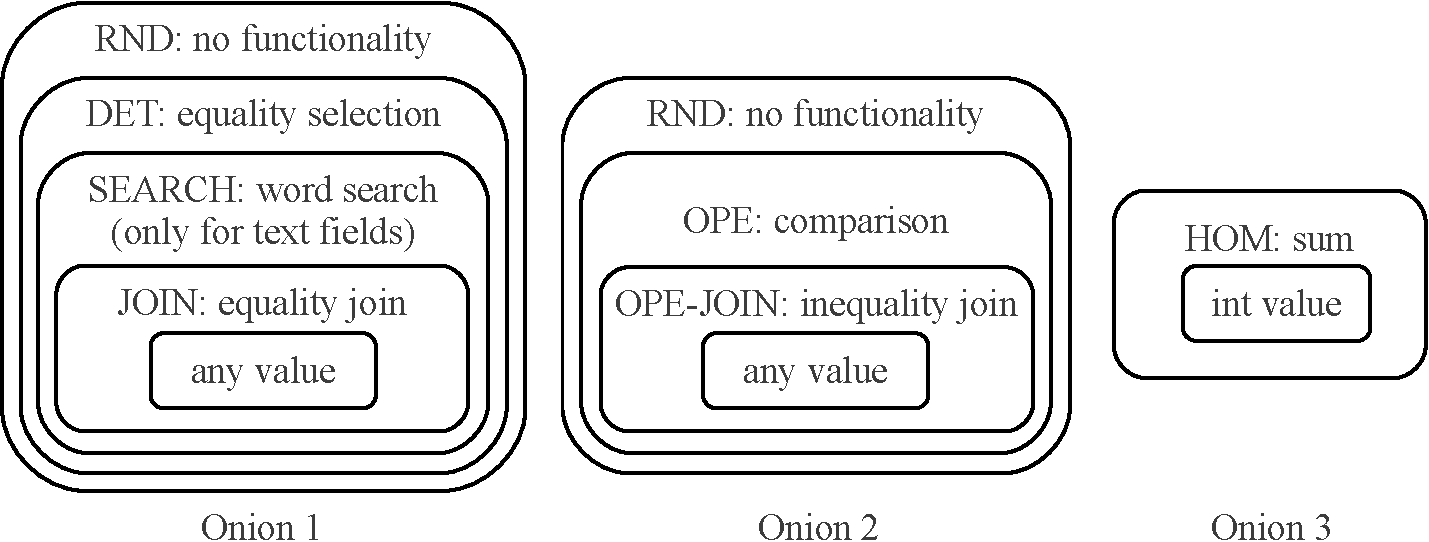
\includegraphics[width=3.1in]{fig/storage.pdf}
\caption{Onion layers of encryption and the classes of computation they allow.}
\label{fig:onion}
\end{figure}

\name{} uses existing transaction and indexing mechanisms in the DBMS
server without any modifications.  For transactions, the proxy passes
along any {\tt BEGIN}, {\tt COMMIT}, and {\tt ABORT} queries to the
DBMS\@.
The DBMS builds indexes of encrypted columns in the same way as it
builds indexes of plaintext data.  The proxy does not request indexes
on $\RND$ encryptions, since no lookups are performed at that level,
but the DB server can construct indexes on $\DET$, $\JOIN$, $\OPE$, and
$\OPEJOIN$ encryptions, as with unencrypted data.
% if the application's schema requested an
% index on the corresponding column (e.g., using an {\tt ALTER} or
% {\tt CREATE} query).

\subsection{Adjustable Query-based Encryption}
\label{ss:onion}

A key part of \name{}'s design is \textit{adjustable query-based
  encryption}, which dynamically adjusts the level of encryption on
the DBMS server.  The goal is provide the most secure encryption
scheme that can also run each query.  For example, if there
is no reason to compare data items in a column, or sort a column, the
column should be encrypted with $\RND$, and for columns that perform
equality checks but not inequality checks, $\DET$ suffices.
Unfortunately, the query set is not always known in advance.
Thus, we need an adaptive scheme that dynamically
adjusts encryption strategies.

Our idea is to encrypt each data item into an \textit{onion}:
each value in the table is dressed in layers of increasingly stronger
encryption, as illustrated in Figs.~\ref{fig:onion} and~\ref{fig:schema}. Each layer of
each onion enables certain kinds of functionality as explained in the
previous subsection.  For example, the outermost layers, $\RND$ and
$\HOM$, provide maximum security, whereas $\OPE$ provides more
functionality.  For numeric values, \name{} maintains three onions,
and for string values, \name{} maintains two onions (the $\DET$ onion,
of the same length as the string, the $\OPE$ onion, of constant length,
and no $\HOM$ onion).

%To prevent the server from learning information from column or table
%names, \name{}'s proxy also anonymizes the schema.

For each level of each onion, the proxy uses the same key for
encrypting values in the same column, and different keys across
columns, onion levels, and tables.  All these keys are derived from
the master key $\mathit{MK}$\@.  For example, for table $t$, column $c$,
encryption level $l$, the proxy uses the key
\begin{equation}\label{eq:columnkey}
K_{t, c, l} = \textrm{PRP}_\mathit{MK} (\mathrm{table}\>t, \mathrm{column}\>c,
    \mathrm{level}\>l),
\end{equation}
where PRP is a pseudorandom permutation (e.g., AES).

Each onion starts out encrypted with the most secure encryption scheme
($\RND$ for onions 1 and 2, and $\HOM$ for onion 3)\@.  As the proxy
receives SQL queries from the application, the onion key manager (OKM)
determines whether layers of encryption need to be removed.  Given a
predicate $P$ on column $c$ needed for the query, the OKM first
establishes what onion layer is needed to perform $P$ on $c$.  If the
encryption of $c$ is not already at an onion layer that allows $P$,
the OKM strips off the onion layers to allow $P$ on $c$, by sending
the corresponding onion key to the server. The lowest encryption level is never stripped.

\name{} implements onion layer decryption using UDFs that run on the
DBMS server.  For example, in Fig.~\ref{fig:schema}, to decrypt onion 2 of column 2 in table 1 
to level $\OPE$, the OKM issues the following query to the server
using the {\tt DECRYPT\_RND} UDF:

\begin{verbatim}
 UPDATE Table1 SET C2-Onion2 =
                   DECRYPT_RND(K, C2-Onion2)
\end{verbatim}
where $K$ is the appropriate key computed as in Eq.
(\ref{eq:columnkey}).

Each constant in a query that is part of a predicate on onion $o$ of column $c$ is encrypted using all onion layers up to the current onion layer of onion $o$ of column $c$. 

Note that onion decryption is performed entirely by the DBMS server.
In the steady state, {\em no server-side decryptions are needed},
because onion decryption happens only when a new type of computation
is performed on a column.  For example, after an equality check is performed
on a column and the server brings the column to level $\DET$, the
column remains in that state, and future queries with equality checks require no decryption.  This property ensures that the
overhead of \name{} is modest in the steady state (see \S\ref{s:eval}) because the server mostly performs typical SQL processing.
The security level to which the database converges is the maximum
privacy level for the set of queries issued by the application.

\begin{figure}[t!] 
\centering
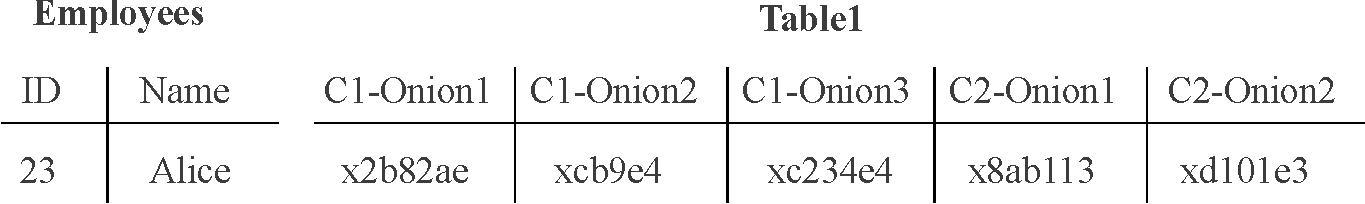
\includegraphics[width=3.1in]{fig/schema.pdf}
\caption{Data layout at the server. When the application creates a
  table with the schema on the left, the table created at the server
  is the one from the right.}
\label{fig:schema}
\end{figure}


\paragraph{Read Query Execution.}

Consider an example consisting of a table \texttt{Employees}, which
has four columns of interest: \texttt{id}, \texttt{name},
\texttt{address}, and {\tt salary}.  Initially, each column in the
table is dressed in all onions of encryption, with $\RND$ and $\HOM$
as outermost layers, as shown in Figure~\ref{fig:onion}.  At this
point, the server can learn nothing about the data content other than
the number of columns, rows, and data size.

To execute predicates on a column, the proxy replaces the column with the
name of the onion that allows the necessary operation on
that field, and, for certain operations (such as {\tt SUM}), the proxy
replaces the operation with its equivalent UDF that operates on
ciphertexts.  

To illustrate when onion layers are removed, consider the query
\texttt{SELECT * FROM Employees WHERE name = 'Alice'}, which requires
lowering encryption of {\tt name} to level $\DET$\@.  In this case,
the proxy first issues the query \texttt{UPDATE Table1 SET C2-Onion1 =
  DECRYPT\_RND($K_{1,2,\RND}$, C2-Onion1)}, and then \texttt{SELECT
  C1-Onion1, C2-Onion1, C3-Onion1, C4-Onion1 FROM Table1 WHERE
  C2-Onion1 = x7d35a3}, where \texttt{x7d35a3} is an encryption of
``Alice'' with key $K_{1,2,\DET}$\ and the keys for lower onion layers.  The proxy decrypts the results
from the server and returns them to the user.

If the next query is {\tt SELECT COUNT(*) FROM Employees WHERE name =
  'Bob'}, no server-side decryptions are necessary, and the proxy
directly issues the query {\tt SELECT COUNT(*) FROM Table1 WHERE
  C2-Onion1 = xbb234a}, where \texttt{xbb234a} is the encryption of ``Bob''.

% Finally, the proxy replaces aggregation operators with equivalent UDFs
% that operate on encrypted values.  For example, if the user issues the
% query {\tt SELECT SUM(salary) FROM Employees}, the proxy rewrites it
% to {\tt SELECT HOM\_AGG(C4-Onion3, PKTABLE.PK) FROM Table2}, where
% {\tt HOM\_AGG} is a UDF that performs Paillier multiplication
% (resulting in addition of plaintexts), {\tt PKTABLE} is a table of
% public keys \name{}{} stores at the server (see
% Fig.~\ref{fig:overview}), and $\PK$ is the Paillier public key
% modulus.


\paragraph{Write Query Execution.}

To support {\tt INSERT}, {\tt DELETE}, and {\tt UPDATE} queries, the
\name{} proxy applies the same processing to the predicates (i.e., the
{\tt WHERE} clause) as for read queries.  {\tt DELETE} queries require
no additional processing.  For all {\tt INSERT} queries and for {\tt
  UPDATE} queries that set the value of a column to a constant, the
proxy encrypts each inserted column's value with each onion layer that
has not been stripped off yet in that column
%For {\tt UPDATE} queries that set the value of a column to a constant,
%the proxy encrypts the value in the appropriate onions as for {\tt
%  INSERT}.

The remaining case is an {\tt UPDATE} that sets a column value based
on another column value, such as {\tt salary=salary+1}.  Such an
update would have to be performed using $\HOM$, to handle additions.
However, in doing so, the values in the $\OPE$ and $\DET$ onions would
become stale.  In fact, an encryption scheme that allows both addition
and comparison at the same time is fundamentally insecure: if a
malicious server knows the order of the items ($\OPE$) and can
increment the value by one, the server can keep adding one to each
field homomorphically until the field becomes equal to some other
value.  This would allow the server to compute the difference between
any two values in the database, which is almost equivalent to knowing
their values.

There are two solutions to this problem.  If a column is incremented
and then only projected (no comparisons performed on it), the solution
is simple: when requesting the value of this field, use the value of
Onion 3 rather than Onion 1 or 2, because Onion 3 is up-to-date.  This
is the case for increment TPC-C queries.
If a column is used in comparisons after it is
incremented, the solution is to split the query into two parts:
a select of the old values to be updated, and an update using
the new values. 
This strategy works well in practice (such as in TPC-C and our benchmark
applications) because updates are typically executed on either individual
rows or a small number of rows.

% removed for space
%.  That is,
% for query \texttt{UPDATE Employees SET salary=salary+1 WHERE id=3},
% the proxy issues the encrypted version of \texttt{SELECT salary FROM
%  Employees WHERE id=3}, and then the encrypted version of
%\texttt{UPDATE Employees SET salary=z WHERE id=3}, where $z$ is one
% more than the result of the first query.\footnote{If the first {\tt
%    SELECT} query returns more than one result, the proxy computes a
%  mapping of old encrypted {\tt salary} values and the corresponding
%  new encrypted {\tt salary} values, and uses a UDF in the second {\tt
%    UPDATE} query to update the {\tt salary} column according to this
%  mapping.}  However, in most cases in practice (such as in TPC-C),
% such updates are executed on individual rows.

\subsection{Computing Joins}
\label{ss:join}

There are two kinds of joins: {\em equi-joins} in which
the join predicate is based on equality, and {\em range joins}, which
involve order checks.
Supporting these joins is a challenging problem.  If two columns are
to be joined, they need to be encrypted with the same key.

% We first describe how \name{} implements
% equi-joins (the overwhelmingly common case, i.e., level
% $\JOIN$), and then describe inequality joins (level $\OPEJOIN$).

%We first describe how \name{} implements equi-joins.  

To provide maximum privacy for equi-joins, the DBMS server should not
be able to join columns for which the user did not request a join, so
columns that are never joined should not be encrypted with the same
keys.  Moreover, if users request a join of columns $A$
and $B$, and a join of columns $C$ and $D$, the DBMS server should not
be able to join $B$ and $C$\@.  Thus, the question is, which keys
should each column be encrypted with, given that we do not know in
advance what columns will be joined?

To address this problem, we introduce a new cryptographic primitive
that allows the DBMS server to dynamically adjust the $\JOIN$
encryption keys of each column.  Each column is initially encrypted
with a different $\JOIN$ key, preventing all joins.  When a query
requests a join, the proxy will give the DBMS server an onion key to
re-encrypt the two columns to the same $\JOIN$ key, allowing joins
between the two columns.

Our algorithm is based on elliptic-curve cryptography (ECC).  When a
row is inserted, the $\JOIN$ encryption of value $v$ is computed as
$\JOIN_K(v) := H(v)^K$, where $K$ is the initial key for that table,
column, and level, and $H$ is a mapping from values (integers or
strings) to a point on an elliptic curve.  When the query joins columns $c$ and
$c'$, the proxy computes $\Delta K=K/K'$, which can be used to bring
the $\JOIN$ encryptions of $c$ and $c'$ to the same key.  Given
$\JOIN_{K'}(v)$ (stored in column $c'$) and $\Delta K$, the DBMS
server uses a UDF to compute $\JOIN_{K'}(v)^{\Delta K} =
H(v)^{K'\times K / K'} = H(v)^K = \JOIN_K(v)$.  Now columns $c$ and
$c'$ share the same $\JOIN$ key, and the DBMS server can perform an
equi-join on $c$ and $c'$ as usual.

We proved the security of this scheme cryptographically (elided here
for space, but will be in an extended version) using the hardness
assumption of computing the discrete logarithm in elliptic curve-based
groups. The server can only join pairs of columns that were joined by
a legitimate query and the encryption scheme does not reveal data.
% 5Intuitively,
% the server cannot perform an equi-join without knowing $K/K'$, and
% $K/K'$ does not reveal any information about either $K$ or $K'$.
% Moreover, the server cannot compute $K$ from $H(v)^K$ because of the
%Given two columns encrypted with $K$
%and $K'$, if the server is not given $K/K'$, it cannot bring the two
%columns to the same encryption level, and thus cannot perform
%unrequested joins.
% We use ECC because of it is
% relatively efficient and ciphertexts are small ($\approx 160$ bits) compared to ciphertexts in
% typical public key cryptosystems for the same security
% level.

% : computing $\JOIN_{K'}(v)^{K/K'}$ is basically a
% multiplication, and does not involve any exponentiation; moreover, ECC

For range joins, a similar dynamic re-encryption scheme is difficult
to construct due to lack of structure of $\OPE$ schemes.  Instead,
\name{} requires that pairs of columns that will be involved in such
joins be declared by the application ahead of time, so that matching
keys are used for level $\OPEJOIN$ of those columns.  Fortunately,
range joins are rare (and not used in any of our example
applications).
%Alternatively, level $\OPEJOIN$
%encryptions can be re-encrypted with matching keys at the expense of
%sending an entire column to the proxy for re-encryption, and then
%sending it back to the DBMS server.

\subsection{Optimizations}
\label{ss:optimize}

\name{} implements four performance optimizations.

\textbf{Insensitive fields.} By default, \name{} encrypts all fields. 
The programmer can annotate just the sensitive fields in the schema
(\S\ref{sec:multi}) to avoid encrypting public fields.

\textbf{Known query set.}  If an application has a known query set or a set of queries likely to happen, as is the case for many web applications, \name{} has a training module that can adjust onions at this level before system startup, thus reducing onion adjustment work from runtime. For a fully known query set, \name{} can also discard any onions that will not be needed (e.g., discard $\OPE$ onion for a column if range queries are not performed on that column).

% For many applications, the queries issued
%by the application are fixed and known ahead of time.  In this case,
% we do not need to adjust onion levels at runtime, and can start the
% database with the exact onion encryption levels that we need.
% Moreover, if a certain column is never used in certain operations, the
%corresponding onion can be omitted altogether.  For example, if an
% application never performs range or order operations on a column, the
% $\OPE$ onion for that column can be omitted.  Discarding onions
% significantly reduces performance costs both in the proxy and in the
% DBMS server.  This optimization is implemented by a \textit{train}
% module in the proxy, which, given a set of queries a user application
% will issue, determines the exact levels of encryption needed.

\textbf{Security convergence.}  Even if the query set is not known in
advance, after an application has run for a considerable time, the
proxy may drop any onions that have not been used, because these
onions are unlikely to be used in the future.  If a query does happen
to use these onions later, the proxy can go through the cost of
adding back the deleted column, but such event should be rare.

\textbf{Ciphertext caching.}  A significant ongoing cost for the proxy
lies in generating $\OPE$ and $\HOM$ encryptions of constants used in
queries.  To avoid this cost, the proxy maintains a cache of
commonly-used constants, along with their encryptions under different
keys.  Since some constants are repeatedly used in queries (e.g.,
the constant 1), this optimization reduces the amount of CPU time
spent by the proxy encrypting data.

\subsection{Discussion}

\name{}'s design supports most relational queries and aggregates on
standard data types, such as integers and text/varchar types.
Additional operations can be added to \name{} by extending its
existing onions, or adding new onions for specific data types (e.g.,
spatial and multi-dimensional range
queries~\cite{multidimRangeQueries}).

There are certain computations \name{} cannot support on encrypted
data. For example, it does not support both computation and comparison
on the same column, such as \texttt{WHERE salary > age*2+10}.  \name{}
can process a part of this query, but it would also require some
processing on the proxy.  In \name{}, such a query should be (1)
rewritten into a sub-query that selects a whole column, \texttt{SELECT
  age*2+10 FROM $\ldots$}, which \name{} computes using $\HOM$, and
(2) re-encrypted in the proxy, creating a new column (call it {\tt
  aux}) on the DBMS server consisting of the newly-encrypted values.
Finally, the original query with the predicate {\tt WHERE salary >
  aux} should be run.  We have not been affected by this limitation in
our test applications (TPC-C, phpBB, HotCRP, and grad-apply).
%Nevertheless, as we will
%see from \S~\ref{s:eval}, \name{}{} supports all queries on TPC-C and
%queries on sensitive data we have encountered in real applications.

%The current \name{} prototype does not support stored procedures or
% other user-defined functions on the server.  Supporting stored
% procedures written in SQL should be straightforward, by having the
% proxy rewrite the SQL statements inside of the stored procedure
%as it would for any other query.  On the other hand, \name{}'s
%design cannot support the execution of arbitrary user-defined
%functions (not written in SQL) over encrypted data.

% \subsection{Access Control}
% 
% Access control can be implemented at the proxy or at a machine between the
% users and the front end. There has been significant work done on such schemes
% which can be used with \name{}. 




% !TEX root = paper.tex

\section{Multiple Principals}
\label{s:multi}
\label{sec:multi}

We now extend the threat model to the case when the application
infrastructure and proxy are untrusted.  This model is especially
relevant for a multi-user web site running a web and application
server.  To explain the problems encountered by a multi-user web
application and \name{}'s solution to these problems, consider phpBB,
a popular online web forum.  Each user has an account and a password,
belongs to certain groups, and can send private messages to other
users. Depending on their groups' permissions, users can read entire
forums, only forum names, or not be able to read a forum at all.

There are several confidentiality guarantees that would be useful
in phpBB\@.  For example, ensuring that a private message sent from
one user to another is not visible to anyone else; ensuring that
posts in a forum are only accessible to users in a group with access
to that forum; and ensuring that the name of a forum is only shown
to users belonging to a group that's allowed to view it.  \name{}
provides these capabilities in the face of arbitrary compromises,
limiting the damage caused by a compromise.

There are two main problems.  First, \name must make it easy to
express policies like the ones above.  Rather than require intrusive
additions to the code, we allow the developer to annotate the database
schema (\S\ref{ss:policy}).  Second, \name must encrypt the data with
several different keys; otherwise, an attacker that compromises the
proxy or application server can decrypt all data.  However, simply
encrypting each data item with a single user's key does not work: in
our example, forum posts must be shared between users, and the set of
users with access to a forum may change at runtime.

Our solution limits the leakage resulting from a compromised
application or proxy to only the data accessible by users who were
logged in during the compromise.  The amount of data leaked
in our solution seems unavoidable given our assumptions about the
impracticality of fully-homomorphic encryption: the relevant data
must be decrypted whenever the web application performs arbitrary
computations to service the requests of active users.

\name{} encrypts different data items with different keys, according
to the specified policies.  \name{} enforces the policies, which
involve multiple users being able to read/write any given data item,
at run-time by encrypting and decrypting the required keys, starting
from the password of the user and ending at the desired keys,
following a chain of keys (\S\ref{ss:keychain}).

%%% The next three paras are the prev version

% We now extend the threat model to the case when the infrastructures
% hosting the application and the proxy are untrusted.  This model is
% especially relevant for a multi-user web site, which in general would
% include a web server and possibly an application server.  If an
% attacker compromises the proxy or the entity querying the DBMS, it can
% gain access to the master key and read all the data.  Our goal is to
% reduce the degree vulnerability so that a compromise doesn't cause as
% much damage.

% Our solution limits the leakage resulting from a compromised
% application or proxy to the data accessible by users who are
% currently active (i.e., logged in after explicit authentication); the
% data belonging to all other users remain protected.  The amount of
% data leaked in our solution seems unavoidable given our assumptions
% and constraints. Because performing arbitrary computations on
% encrypted data, which required fully-homomorphic encryption, is
% currently neither practical nor believed to become practical
% soon~\cite{trillion}, the relevant data should be decrypted whenever
% the web application needs to perform arbitrary operations (as is the
% case in general) to service the requests of active users.

% \name{} replaces the proxy's master key with multiple different keys
% and encrypts different data items with different keys, according to
% policies expressed over the database schema by the application
% developer (\S\ref{ss:policy}).  Then, \name{} enforces the policies at
% run-time by encrypting and decrypting the required keys, starting from
% the password of the user and ending at the desired keys, following a
% ``chain'' of keys (\S\ref{ss:keychain}).


% The solution is to replace the \frontend{}'s master key with many
% ``client keys'': each client of the application stores a client key,
% which only enables the client to access the data it is entitled to
% according to application logic. To enable the application to perform
% arbitrary computation on user data, each client gives its key to
% \name's \frontend{} for the duration of its session. Therefore, if an
% adversary compromises the application, he can only read the data of
% clients that are currently active; the data belonging to the other
% clients remains protected.


% TODO: in Facebook users are logged in all the time, so maybe we want
% to do this at the granularity of sessions


\subsection{Policy Annotations}
\label{ss:policy}

To express the privacy policy of a database-backed application at the
level of SQL queries, the application developer can annotate the
schema of a database in \name{} by specifying, for each subset of data
items, which {\em principal} has access to them.  A principal is an
entity, such as a user or a group, over which it is natural to specify
an access policy.  Each SQL query involving an annotated data item
requires the privilege of the corresponding principal. 

% \name relies on the notion of a {\em principal}, an entity involved in
% access control, for example, a user or a group.  Private data items in
% an SQL database can be marked as accessible only to a particular
% principal, and each SQL query involving the private data item requires
% the privilege of that principal. Programmers express the policy of
% their application in terms of principals, by annotating their SQL
% schema in four steps, 

An application developer annotates the schema using the steps
described below and shown in Figure~\ref{fig:privmsg}.

\renewcommand{\FrameSep}{0.05in}
\begin{figure}[t!]
\begin{framed}
\footnotesize

\begin{tabbing}
{\bf PRINC TYPES physical\_user EXTERNAL;} \\
{\bf PRINC TYPES user, msg;} \\
\\

x \= msgtext \= varchar(255) \= \kill

CREATE TABLE privmsgs (\\
\> msgid \> int, \\
\> subject \> varchar(255) \> {\bf ENC\_FOR PRINC msgid TYPE msg}, \\
\> msgtext \> text \> {\bf ENC\_FOR PRINC msgid TYPE msg} ); \\
\\

CREATE TABLE privmsgs\_to (\\
\> msgid int, ~ rcpt\_id int, ~ sender\_id int, \\

\> {\bf PRINC sender\_id TYPE user} \\
\> {\bf ~ ~ ~ HAS\_ACCESS\_TO PRINC msgid TYPE msg}, \\
\> {\bf PRINC rcpt\_id TYPE user} \\
\> {\bf ~ ~ ~ HAS\_ACCESS\_TO PRINC msgid TYPE msg}); \\
\\

x \= sender\_id  int, x \= username varchar(255), x \= sender\_id text \= \kill

CREATE TABLE users (\\
 \> userid int, ~ username varchar(255), \\

\> {\bf PRINC username TYPE physical\_user HAS\_ACCESS\_TO} \\
\> {\bf ~ ~ ~ PRINC userid TYPE user}); 

\end{tabbing}

\vspace{-4mm}
\hrulefill
\vspace{-2mm}

\begin{center}
\textit{Example table contents, without anonymized column names:}
\end{center}
 \hspace{1mm}
 \begin{minipage}[h]{1.7 in}
  \centering
  \begin{tabular}{p{0.8cm}|p{1cm}|p{0.8cm}}
  msgid & subject & msgtext \\ \hline
  5 & xcc82fa & x37a21f \\ 
  \end{tabular}

  \smallskip

  \begin{tabular}{p{0.8cm}|p{1cm}|p{0.8cm}}
  msgid & rcpt\_id  & sender\_id \\ \hline
  5 & 1 & 2 \\ 
  \end{tabular}
\end{minipage}
\hspace{0mm}
\begin{minipage}[h]{0.9in}
 \centering
  \begin{tabular}{c|c}
  userid & username \\ \hline
  1 & `Alice'  \\  
  2 & `Bob' 
  \end{tabular}
 \end{minipage}
\end{framed}

\caption{
Part of phpBB's schema with annotations to secure private messages.
Only the sender and receiver may see the private message. An attacker
that gains complete access to phpBB and the DBMS can access
private messages of only currently active users.  Bold text indicates
annotations added for \name.
    }
\label{fig:privmsg}
\end{figure}

{\em Step 1.} The developer must define the {\em principal types}
({\small \tt PRINC TYPES}) used in her application, such as users,
groups, or messages.  A {\em principal} is an instance of a principal
type, e.g., principal 5 of type user.  Principals are of two types:
external and internal. External principals correspond to end users who
explicitly authenticate themselves to the web site using a password.
When a user logs into the application, the application must provide
the user password to the \name proxy so that the user can get the
privileges of his external principal.  Privileges of other (internal)
principals can only be acquired through delegation, as described in
the Step 3.  The application also informs the proxy when the user logs
out.

{\em Step 2.} The developer must specify which columns in her SQL
schema contain sensitive data, along with the principals that should
have access to that data, using the {\tt \small ENC\_FOR}
annotation.  \name requires that for each private data item in a row,
the name of the principal that should have access to that data be
stored in another column in the same row.
% That principal is typically a (primary) key column of the table.
For example, in Figure~\ref{fig:privmsg}, the decryption of {\em msgtext}
\texttt{x37a21f} is only available to principal 5 of type {\em msg}.

{\em Step 3.}  Programmers can specify rules for how to delegate the
privileges of one principal to other principals.  For example, in
phpBB, a user should also have the privileges of the groups he belongs
to.  Since many applications store such information in tables,
programmers can tell \name to infer delegations from rows in an
existing table.  In \name, programmers can annotate a table $T$ with
{\tt \small PRINC $a$ TYPE $x$ HAS\_ACCESS\_TO PRINC $b$ TYPE $y$}.
This annotation indicates that each row present in that table grants
principal $a$ of type $x$ access to everything that principal $b$ of
type $y$ can access.  Here, $x$ and $y$ must always be fixed principal
types.  Principal $b$ is always specified by the name of a column in
table $T$.  On the other hand, $a$ can be either the name of another
column in the same table, a constant, or $T2.\textrm{col}$, meaning {\em all}
principals from column $\textrm{col}$ of table $T2$.  For example, in
Figure~\ref{fig:privmsg}, principal ``Bob'' of type {\em
  physical\_user} has access to principal 2 of type {\em user}, and
in Figure~\ref{fig:hotcrp}, all principals in the {\em contactId}
column from table {\em PCMember} (of type {\em contact}) have access
to the {\em paperId} principal of type {\em review}.  Optionally, the
programmer can specify a predicate, whose inputs are values in the
same row, to specify a condition under which delegation should occur,
such as excluding conflicts in Figure~\ref{fig:hotcrp}.
\S\ref{s:apps} provides more examples of using annotations to secure
real applications.


%The task of the developer only consists of annotating the schema and
%informing \name's \frontend{} of when users login (and providing their
%passwords) and logout. 

To aid debugging, we allow the developer to provide a SQL trace of a
previous run of the application that also includes when users logged
in or out, and the proxy can verify if previous queries are permitted
to run given the current annotations, and flag whether the developer
should revise the annotations.

% \name{} needs to know what clients should have access to what data
% from the database in order to encrypt the data with appropriate keys.
% Since such policy is dictated by application logic, the programmer of
% the application should specify such policy.

% We provide a simple \textit{annotation scheme} using which \textit{the
% programmer can annotate the schema of the tables} in the DB. We show
% how a programmer can naturally express application access control to
% the data in the database using this scheme.

% The programmer should annotate any column whose data items are involved
% in access control. There are four types of annotations, which we will
% exemplify with a real scenario from phpBB in Figure~\ref{fig:privmsg}.

% \noindent -- \pr{}: denotes any class of entities involved in access
% control. Annotating column $c$ with \pr{} $P$ denotes that each item in
% column $c$ is an instance of a principal of type $P$. In our examples,
% principals are users and messages. For instance, column users.userid
% contains principal user instances $1$ and $2$. A column can be annotated
% with multiple principals (see \S\ref{s:apps}).

% \noindent -- $c$\ \encfor\ $P$: stands for \textit{encrypted for}
% principal $P$. There must be a column annotated with principal $P$
% in the same table. Each data item in column $c$ will be encrypted and
% only accessible to the instance of principal $P$ in the same row. For
% example, msgtext  x37a21f6732 can only be decrypted by Principal msg
% 5. Any number of columns can be encrypted for the same principal, such
% as msgtext and msgsubject.

% \noindent -- $P_1$ \access{} $P_2$, where $P_1$ and $P_2$ are principal
% annotations in the same table, denotes that each instance of  principal
% $P_1$ has access to anything that the instance of principal $P_2$ in the
% same row has access. An annotation for principal $P_2$ must be present
% in the same table.  For example, in table privmsgs\und{}to, principal
% user 1 and 2 have access to anything that principal msg 5 has access.

% \noindent -- \gives{} P: is added to a column containing names of clients
% or other physical entities who will be providing a password when they
% login to the system. Each password will be used for the instance of
% principal $P$ in the same row. For example, in table users, when Alice
% logs in, her password will be used for Principal user 1.

% Two principal instances from two different tables are equal if they are
% of the same type and have equal value.

% A client Alice has access to data item $d$ in column  $c$ if there is
% a valid path from the \gives{} record corresponding to Alice to the
% principal instance for which $d$ was encrypted. A valid path consists
% of \access{} links in the same row of a table or equality of principal
% instances across different tables. We can see both Alice and Bob have
% access to decrypt msgtext x37a21f6732, but, say a third user Chris with
% userid 3, would not have access to the data.

% To support more general policies, \name{} allows ``conditional'' \access{}
% annotations: \access{} followed by ``if Pred()'', where Pred() is a
% boolean SQL user-defined function by the programmer taking as input a
% row of the table on which it is defined. \name{} evaluates Pred() on
% each row; for the rows where Pred() is true, \name{} grants the access
% in question to the principal instances in that row. Inside Pred(),
% the programmer can perform arbitrary SQL queries.

% For sophisticated access control schemes, Pred() may contain SQL queries
% touching principals in another table, say $t$. At some later time, after
% access is given, an application administrator may change certain values
% in $t$ and the value of the predicate may change. \name{} thus must
% re-evaluate the predicate for each of the specific principals affected
% by the administrator's change. However, such changes may never occur
% (for applications who setup the access control policy at system setup)
% such as HotCRP or they can happen rarely (e.g., when the administrator
% bans a user) as in phpBB.

% The only changes needed to the application are such schema annotations
% (and any predicates' definitions) and authentication: the application
% should inform \name when a user logs in or out and provide it with
% the password (implemented via simple INSERT or DELETE from a fake table).

% \S\ref{s:apps} provides more examples of using annotations to secure
% real applications.

\subsection{Key Chaining}
\label{ss:keychain}

Each principal (i.e., each instance of each principal type) is associated
with a secret, randomly-chosen key.  If principal B has access to
principal A, then principal A's key is encrypted using principal B's
key, and stored in a special \textsf{access\_keys} table in the database.
In this way, principal B has access to principal A's key.  For example,
in Figure~\ref{fig:privmsg}, to give users 1 and 2 access to message 5,
the key of {\em msg} 5 is encrypted with the key of {\em user} 1, and
also separately encrypted with the key of {\em user} 2; both encryptions
are stored in \textsf{access\_keys}.  Each sensitive
field is encrypted with the key of the principal in the {\small \tt
ENC\_FOR} annotation. \name{} encrypts the sensitive field with
onions in the same way as for single-principal \name,
except that onion keys are derived from a principal's key as opposed to
a global master key.

The key of each principal is  a combination of a symmetric key
and a public--private key pair.  In the common case, \name uses the
symmetric key of a principal to encrypt any data and other principals'
keys accessible to this principal, with little CPU cost.  However, this is not always
possible, if some principal is not currently online.  For example,
in Figure~\ref{fig:privmsg}, suppose Bob sends message 5 to Alice, but
Alice (user 1) is not online.  This means that \name does not have access
to user 1's key, so it will not be able to encrypt message 5's key with
user 1's symmetric key.  In this case, \name looks up the public key
of the principal (i.e., user 1) in a second table, \textsf{public\_keys}, and encrypts
message 5's key using user 1's public key.  When user 1 logs in, they
will be able to use the secret key part of their key to decrypt the
key for message 5.

For external principals (e.g., physical users), \name assigns a
random key just as for any other principal.  To give an external user
access to the corresponding key on login, \name stores the key of each
external principal in a third table, \textsf{external\_keys}, encrypted
with the principal's password.  This allows \name to obtain a user's
key given the user's password, and also allows a user to change his or
her password without changing the key of the principal.

In \name{}, one user can grant a second user access to principal $P$
only if the first user already has access to $P$ himself.  At the
cryptographic level, this means that the first user must have $P$'s
key in order to re-encrypt it for the second user.  This closely
follows real-world semantics, since if someone can grant others
access to $P$, they can also grant themselves access to $P$.

When encrypting data in a query or decrypting data from a result,
\name{} follows key chains starting from passwords of users logged in
until it obtains the desired keys. As an optimization, when a user
logs in, \name{}'s proxy loads the keys of some principals to which
the user has access (in particular, those principal types that do not
have too many principal instances---e.g., for groups the user is in,
but not for messages the user received---which \name determines by
keeping aggregate statistics).

Applications inform \name{} of a user logging in or out by simply
issuing SQL {\tt INSERT} and {\tt DELETE} queries to a special table
\textsf{cryptdb\_active}, which the proxy recognizes.

\name{} guards the data of inactive users at the time of an
attack. However, some special users such as administrators with access
to a large pool of data enable a larger compromise upon an attack.  To
avoid attacks happening when the administrator is logged in, the
administrator should create a separate user account with restricted
permissions when accessing the application as a regular user. Also, as
best practice, an application should automatically log off users who
have been inactive for a while.

% In a more complex access control scheme, the programmer might define an SQL predicate for the \small{HAS\_ACCESS\_TO} annotation to touch rows outside of the current row or table. If those tables or rows are changed dynamically (for example, when an administrator changes access control), \name must re-evaluate the predicate for the specific principals involved and add or remove access to relations; however, this case either did not happen in the real applications we evaluated or it happened rarely.

%EVEN say about the predicate being reevaluated??



% TO explain: join operations on columns with differntely encrypted data
% --  only on behalf of a person -- in general if a person has access it
% can be performed

%\subsection{Discussion}


% When the administrator needs
% to use the more powerful account for rare permissions changes or other
% management, the administrator should login at arbitrary times and,
% whenever possible, to make the website unavailable for maintenance for
% a short period of time at a time when it likely is not used.

%Passive attackers snooping on data may try to collect data
%of many users that log in over a period of time.  However, the
%first time \name's proxy receives a query for which it does not
%have sufficient keys, such as in an SQL injection attack, the
%proxy reports it as an attack.  If the administrator reacts quickly,
%the opportunity for the attacker to collect
%confidential data will be greatly reduced.


% !TEX root = paper.tex

\section{Application Case Studies}
\label{s:apps}

In this section, we explain how \name can be used to secure three
existing multi-user web applications.  In our examples, annotations
are shown in bold.  For brevity, we show simplified schemas, ignoring
irrelevant fields and type specifiers.  Overall, we find that once the
programmer specifies the principals in the application's schema, and
the delegation rules for them using {\small \tt HAS\_ACCESS\_TO},
protecting additional sensitive fields just requires additional
{\small \tt ENCRYPT\_FOR} annotations.

{\bf phpBB} is a widely-used open source forum with a rich set of
access control settings. Users are organized in groups; both users and
groups have a variety of access permissions that the application
administrator can choose. We already showed how to secure private
messages between two users in phpBB in Fig.~\ref{fig:privmsg}.  A more
interesting case is securing access to posts, as shown in
Fig.~\ref{fig:posts}.  This example shows how to use predicates
(e.g., {\small \tt IF optionid=...}) to give conditional access to
principals, and also how one column ({\tt forumid}) can be used to
represent multiple principals (of different type) with different
privileges.  There are more ways to access to a post, but we do not
show them all here for brevity.

% phpBB example

\renewcommand{\FrameSep}{0.05in}
\begin{figure}[t!]
\begin{framed}
\footnotesize

\begin{tabbing}

{\bf PRINC TYPES physical\_user EXTERNAL;} \\
{\bf PRINC TYPES user, group, forum\_post, forum\_name;}\\

\\

x \= \kill

CREATE TABLE users ( userid int, username varchar(255),\\

\> {\bf PRINC username TYPE physical\_user HAS\_ACCESS\_TO } \\
\> {\bf ~ ~ ~ PRINC userid TYPE user});\\

\\

CREATE TABLE usergroup ( userid int, groupid int,\\

\> {\bf PRINC userid TYPE user HAS\_ACCESS\_TO } \\
\> {~ ~ ~ \bf PRINC groupid TYPE group});\\

\\

CREATE TABLE aclgroups ( groupid int, forumid int, optionid int, \\

\> {\bf PRINC groupid TYPE group HAS\_ACCESS\_TO }\\
\> {\bf ~ ~ ~ PRINC forumid TYPE forum\_post IF optionid=20}, \\
\> {\bf PRINC groupid TYPE group HAS\_ACCESS\_TO }\\
\> {\bf ~ ~ ~ PRINC forumid TYPE forum\_name IF optionid=14}); \\

\\
x \= \kill


CREATE TABLE posts ( postid int, forumid int,\\
\> post text {\bf ENCRYPT\_FOR PRINC forumid TYPE forum\_post});\\
\\
CREATE TABLE forum ( forumid int,\\
\> name varchar(255) {\bf ENCRYPT\_FOR PRINC forumid } \\
\> {\bf ~ ~ ~ TYPE forum\_name});

\end{tabbing}
\vspace{-0.15in}

\end{framed}

\vspace{-0.2in}
\caption{Annotated schema for securing access to posts in phpBB\@. A
  user has access to see the content of posts in a forum if any of the
  groups that the user is part of has such permissions, which is indicated
  by optionid $20$ in the aclgroups table for the corresponding forumid
  and groupid. Similarly, optionid 14 enables users to see the forum's
  name.}

\label{fig:posts}
\end{figure}

% HOTCRP

{\bf HotCRP} is a popular conference review application.  A key policy
for HotCRP is that PC members cannot see who reviewed their own (or
conflicted) papers.  Fig.~\ref{fig:hotcrp} shows \name annotations for
HotCRP's schema to enforce this policy.  Today, HotCRP cannot prevent
a curious or careless PC chair from logging into the database server
and seeing who wrote each review for a paper that he is in conflict
with.  As a result, conferences often set up a second server to review
the chair's papers or use inconvenient out-of-band emails.  With
\name, a PC chair cannot learn who wrote each review for his paper,
even if he breaks into the application or database, since he does not
have the decryption key.\footnote{Fully implementing this policy would
  require setting up two PC chairs: a main chair, and a backup chair
  responsible for reviews of the main chair's papers.  HotCRP allows
  the PC chair to impersonate other PC members, so \name annotations
  would be used to prevent the main chair from gaining access to keys
  of reviewers assigned to his paper.} (We assume the PC chair is not
malicious, but might be careless, so he won't modify the application
to log the passwords of PC members to subvert the system.)


{\bf grad-apply} is a graduate admissions system used at a major
university.  We annotated its schema to allow an applicant's folder to be accessed only by the respective applicant and any faculty using: 
 {\tt \small PRINC reviewers.reviewer\_id TYPE reviewer} (meaning all reviewers) {\tt \small HAS\_ACCESS\_TO candidate\_id} in table candidates, and {\tt \small HAS\_ACCESS\_TO letter\_id} in table letters. The applicant can see all his folder except for letters of recommendation.  Overall, grad-apply has simple access control and therefore simple
annotations. 


%\begin{figure}
%\renewcommand{\FrameSep}{0.05in}
%\begin{framed}
%\footnotesize
%
%{\bf PRINC TYPES physical\_contact EXTERNAL;} \\
%{\bf PRINC TYPES contact, paper;}
%
%\begin{tabbing}
%
%x \= \kill
%
%CREATE TABLE ContactInfo ( contactId int, email varchar(120), \\
%
%\> {\bf PRINC email TYPE physical\_contact HAS\_ACCESS\_TO PRINC contactId TYPE contact});\\
%
%\\
%
%CREATE TABLE PaperConflict( paperId int, contactId int);\\
%\\
%
%{\bf NoConflict(paperId, contactId):} \\
%\> {\bf (SELECT count(*) FROM PaperConflict c WHERE c.paperId = paperId AND c.contactId = contactId)=0; } \\
%
%\\
%
%CREATE TABLE PaperReview ( paperId int, \\
%\> contactId int {\bf ENCRYPT\_FOR PRINC paperId TYPE paper}, \\
%\> commentsToPC text {\bf ENCRYPT\_FOR PRINC paperId TYPE paper},\\
%\> {\bf PRINC contactId TYPE contact HAS\_ACCESS\_TO PRINC paperId TYPE paper  IF NoConflict(paperId, contactId)} \\
%
%\end{tabbing}
%
%\end{framed}
%
%\caption{
%      Annotated schema for securing reviews in HotCRP\@. Reviews and the identity of reviewers providing the review will only be available to assigned reviewers who are not conflicted even if these reviewers are PC Chairs.}
%\label{fig:posts}
%\end{figure}

%HOTCRP any PC member can see reviews of a paper and who reviewed it other than conflicted PC members or PC Chairs

\begin{figure}
\renewcommand{\FrameSep}{0.05in}
\begin{framed}
\footnotesize

{\bf PRINC TYPES physical\_contact EXTERNAL;} \\
{\bf PRINC TYPES contact, review;}

\begin{tabbing}

x \= \kill


CREATE TABLE ContactInfo ( contactId int, email varchar(120), \\
\> {\bf PRINC email TYPE physical\_contact HAS\_ACCESS\_TO } \\
\> {\bf ~ ~ ~ PRINC contactId TYPE contact});\\

\\

CREATE TABLE PCMember ( contactId int ); \\

CREATE TABLE PaperConflict ( paperId int, contactId int );\\
\\

{\bf NoConflict (paperId, contactId):} ~ ~ ~ ~ ~ ~ {\tt /*} Define a SQL function {\tt */} \\
\> {\bf (SELECT count(*) FROM PaperConflict c  WHERE }\\
\> {~ ~ ~ \bf c.paperId = paperId AND c.contactId = contactId) = 0;} \\

x \= commentsToPC \= text \= {\bf ENCRYPT\_FOR PRINC paperId TYPE review} \= \kill
\\
CREATE TABLE PaperReview ( paperId int, \\
\> reviewerId \> int \> {\bf ENCRYPT\_FOR PRINC paperId TYPE review}, \\
\> commentsToPC \>text \> {\bf ENCRYPT\_FOR PRINC paperId TYPE review},\\


\> {\bf PRINC PCMember.contactId TYPE contact }\\
\> {\bf ~ ~ ~ HAS\_ACCESS\_TO PRINC paperId TYPE review IF } \\
\> {\bf ~ ~  ~ ~ ~ ~ ~ ~ ~ ~ ~ ~ ~ ~ ~ ~ ~ NoConflict(paperId, contactId)});

\end{tabbing}
\vspace{-0.15in}
\end{framed}
\vspace{-0.2in}
\caption{Annotated schema for securing reviews in HotCRP\@. Reviews and
the identity of reviewers providing the review will only be available to
PC members (table PCMember includes PC Chairs) who are not conflicted,
and PC Chairs cannot override this restriction.}

\label{fig:hotcrp}
\end{figure}




% !TEX root = paper.tex

\section{Implementation}
\label{s:impl}

The \name{} proxy consists of a C++ and a Lua module.  The C++ module
consists of a query parser; a query encryptor and rewriter, which
encrypts fields or calls UDFs; and a result decryption module.  To
allow applications to transparently use \name, we used MySQL Proxy and
implemented a Lua module that passes queries and results through our
C++ module.  We implemented our new cryptographic protocols using
NTL~\cite{shoup:ntl}.  \name{} is $\sim$8500 non-empty lines of code.

\name is portable and supports both Postgres 9.0 and MySQL 5.1;
initially implemented in Postgres, porting \name{} to MySQL required
changing only 86 lines of code, mostly in the code for connecting to the
MySQL server and declaring UDFs.  As mentioned earlier, \name{} does not
change the DBMS; we implement all server-side functionality with
UDFs and server-side tables.  This modular change was possible because
the DBMS lies in between two aspects of query processing that \name{}
must modify: query planning and execution is between query parsing
and low-level operations on data items.
\name should run on top of any SQL DBMS that supports UDFs.

% by rewriting queries in the proxy and replacing individual operations
% through UDFs.


 
% !TEX root = paper.tex


\begin{figure*}
\small
\centering
\begin{tabular}{c|ccl}
\bf Application & \multicolumn{1}{c}{\bf Annotations} & \bf Login/logout code & \bf Sensitive fields secured, and examples of such fields \\
\hline
\centering phpBB 	& 32 (11 unique) & 	7 lines	& 24: private messages (content, subject), posts, forums \\
\centering HotCRP 	& 29 (12 unique)	& 	2 lines	& 22:  paper content and paper information, reviews \\
\centering grad-apply & 106 (13 unique) &  2 lines & 98: student grades (61), scores (17), recommendations, reviews \\
TPC-C {\scriptsize (single princ.)} & 0	&		0		&	92: all the fields in all the tables encrypted \\
\end{tabular}
\caption{Effectiveness of annotations and fields secured. This table shows, for 4 different applications, the number of annotations the programmer needs to add to secure sensitive fields, lines of code to be added to provide \name{} with the password of users, and the number of sensitive fields that \name{} secures with these annotations. We count as one annotation any invocation of our three types of annotations and any line of any SQL predicate used in a {\tt \small HAS\_ACCESS\_TO} annotation. Since multiple fields in the same table are usually encrypted for the same principal (e.g., message subject and content), we also report unique annotations. }
\label{fig:annotations}
\end{figure*}

\section{Experimental Evaluation}
\label{s:eval}


This section evaluates the security \name{} provides to applications,  developer effort to annotate the schema, as well as
performance overheads. 
%rest of this section show that \name has low runtime overheads
%(on the order of 27\% throughput cost and 0.64~ms latency
%cost for TPC-C queries), is easy to port to new DBMS servers,
%and requires no application code changes.
Our multi-user application evaluations are done with phpBB, HotCRP,
and grad-apply (\S\ref{s:apps}).  We annotate all sensitive fields in these applications so that they are encrypted.To study the performance of our encrypted DBMS, we also measure the query and
transaction throughput for the industry-standard TPC-C benchmark and
its SQL operators. For TPC-C, we run in single-principal mode, which means that all data (even insensitive) is encrypted and all queries are performed on encrypted data. 

% may want to say that it captured apps properly

% OUR SUMMARY
%Results show that \name incurs a throughput overhead of
%13\% for phpBB and 27\% for TPC-C which we consider acceptable considering the added confidentiality, requires 11--13 lines of unique annotations to secure more than twice as many sensitive fields in multi-user applications, due to adjustable query-based encryption keeps almost all sensitive fields encrypted with $\RND$, and supports all queries on TPC-C and  on three applications.
%the most secure encryption scheme.

% We evaluate the performance of the encrypted DBMS on TPC-C, a standard
% SQL benchmark. For TPC-C, \name{} operates in single-principal
% mode. In this mode, all the data in the DB is encrypted (for one
% principal) and applications can run on top of \name{} unchanged with
% no annotations. The TPC-C evaluation enables useful microbenchmark
% evaluation and gives us the worst-case performance of the DBMS: when
% all fields (even insensitive ones) are encrypted: The throughput loss
% is only 27\% and a latency addition of 0.64ms.

\subsection{Application Security and Annotations}

The first observation from porting TPC-C, phpBB, HotCRP, and grad-apply, is that \name{} supports, on encrypted data, all queries from TPC-C and all queries on sensitive fields from our three applications. Equally important, our annotations were able to secure sensitive fields in the three applications without limiting these applications' functionality. 

Figure~\ref{fig:annotations} shows the effectiveness of annotations
and fields secured for our applications.  Overall, \name requires few
unique annotations, and minimal changes to the application code.  Part of
the simplicity comes from the fact that usually only one annotation is
needed to secure one additional column.  For TPC-C, no annotations or
application changes were required, because TPC-C ran in single-principal
mode (corresponding to threat 1 from \S\ref{ss:dbthreat}): the entire
database was encrypted with the key of one principal single key.

% To demonstrate the portability of existing applications to
% \name, we ran several applications on \name,
% including TPC-C and two different versions of an academic institution's 
% graduate admissions web application, one written using hand-written SQL
% queries and one
% written using the Django ORM system~\cite{bib:django} for Python.  \name
% was able to support all SQL queries from these applications without having
% to modify the queries or the application in any way. 

\begin{table}
\begin{tabular}{@{}c|c|c|c||c||c@{}}
\bf Application & 	\bf $\RND$ & 	\bf $\DET$ & 	\bf $\OPE$ & 	\bf Total & 	$\HOM$ \\
\hline
PhpBB &          19   &   		 2    &    		 3$^*$  &   		 24 & 		2  \\
HotCRP &	 	19 & 		1 & 			2$^*$ & 	 		22 &  	2 \\
grad-apply & 	 89& 		7  & 			2$^*$  & 		98 &  	0 \\
TPC-C & 		65 & 		19 &  		8$^*$ & 			92 & 		8
\end{tabular}
\caption{Steady-state security of onion layers. Each number indicates how many encrypted fields remain at that onion level after the applications issued all query types. $\DET$ includes $\JOIN$ values because they have similar security level (AES). Each field is counted for the onion layer with lowest security. We also report how many fields in addition used the $\HOM$ onion. (*) All the fields at $\OPE$ were only slightly sensitive (e.g., post\_time, number of forum posts).} 
\label{t:onion}
\end{table}



To quantify the security level provided by \name to these
applications, Table~\ref{t:onion} shows the encryption schemes that
are exposed to the server for each application in steady-state under a
typical workload.  The results show that most fields (71--91\%) remain
encrypted with $\RND$, the most secure scheme. Looking at the most
sensitive fields in each application, they were all at $\RND$. $\DET$,
which leaks only information about repeating values, is used in
5\%--21\% of the fields.  $\OPE$, which leaks order, is used a little
less frequently (9--13\%), and only for fields that are marginally
sensitive (e.g., timestamps).  Thus, \name's adjustable security
provides a significant improvement in confidentiality over revealing
all encryption schemes to the server.

Finally, we empirically validated \name's confidentiality guarantees
by trying real attacks on phpBB that have been listed in the CVE
database~\cite{cve:stats}, including two SQL injection attacks
(CVE-2009-3052 \& CVE-2008-6314), bugs in permission checks
(CVE-2010-1627 \& CVE-2008-7143), and a bug in remote PHP file
inclusion (CVE-2008-6377).  We found that, for users not currently
logged in, the answers returned from the DBMS were encrypted; even
with root access to the application server, proxy, and DBMS, the
answers were not decryptable.

\subsection{Performance Results}

To evaluate the performance of \name, we use a server with an Intel
Xeon 4-core 3.20~GHz CPU and 3~GB of RAM, and a machine with
an Intel Xeon 4-core 1.6~GHz E7310 CPU and 8~GB RAM to
simulate multiple users.

\subsubsection{TPC-C}

% We report the throughput and latency of \name proxying a Postgres DBMS
% server and compare it to vanilla Postgres for TPC-C, an
% order-processing benchmark.

% trace.
% Rather than just run the TPC-C benchmark, we generate a mix of random
% OLTP queries by collecting TPC-C execution traces and then having
% multiple clients present these queries to \name.  This approach
% allows us to evaluate the performance overhead of \name on a variety
% of random OLTP-like access patterns.

We compare the performance of TPC-C running on Postgres with its
performance when using a \name proxy in front of a Postgres server.
Figures~\ref{fig:querytputlat} and \ref{fig:trantput} shows the
query throughput on TPC-C when transactions are disabled and enabled,
respectively.  \name incurs a 21\% overhead without transactions, and
the overhead with transactions increases to 27\% because of
increased lock contention caused by longer processing times and
expanded queries.

%Note that because of the CPU cost of encrypting data
%in the proxy, unoptimized \name{} requires more clients (running on
%different cores) to achieve maximum throughput.

%To measure the query processing throughput of \name{}, we first report
%the throughput for TPC-C queries when transactions are not used, as
%shown in Figure~\ref{fig:querytputlat}.  We can see that \name incurs
%a throughput reduction of 21\% compared to an unmodified Postgres
%server (based on the highest throughput for both configurations).

\begin{figure*}[t!]
\begin{minipage}[t]{4.4in}
\centering
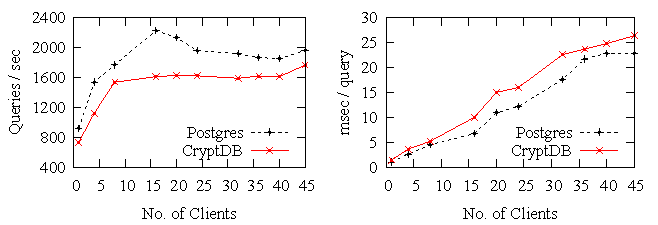
\includegraphics{fig/queries.pdf}
\caption{Throughput and latency for TPC-C queries without transactions.}
\label{fig:querytputlat}
\end{minipage}
\begin{minipage}[t]{2.2in}
\centering
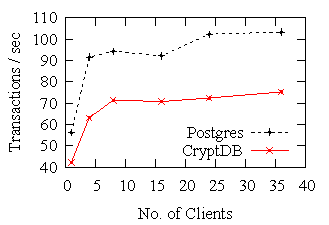
\includegraphics{fig/trantput.pdf}
\caption{Throughput of TPC-C transactions.}
\label{fig:trantput}
\end{minipage}
\end{figure*}

% In case of unoptimized \name, client-side
% processing times for each query are increased even further,
% leading to significantly more transaction conflicts and an
% overall throughput reduction of 70\%.

To understand the sources of \name's overhead, we examine the
throughput of individual SQL operators; this analysis is useful
because the mix of operators changes with application.  For each
operator, we collect the corresponding queries from TPC-C, and
measure the latency for those queries running under \name and under
Postgres.  Table~\ref{t:microlat} shows the results.
The proxy encryption time adds an average of 0.34~ms to the query.
The ciphertext caching optimization masks the high latency of queries
requiring $\OPE$ and $\HOM$, as indicated by bold numbers and their
corresponding Proxy$^-$ values.
The DBMS server latencies with and without \name are similar,
suggesting that the expansion of data at the server caused by encryption has a small
impact.
End-to-end, \name with the caching optimization adds
0.64~ms of latency to each query.

Figure~\ref{fig:microtput} shows the throughput for the same mix of
queries for Postgres, \name, and a strawman design that performs each
query by first decrypting the data using a UDF, performing the query,
and re-encrypting the result (if updating the row).  In all cases
except for insert, the strawman performs significantly worse than
\name, since the DBMS cannot use an index to satisfy WHERE clauses. It
is indeed an unexpected fact that the higher security of \name{} over
the strawman in fact also brings better performance. For six SQL
operators (Select equality, Select join, Select range, Delete, Insert,
and Update set), the throughput overhead of \name is negligible
compared to Postgres.  These six constitute most of the queries for
TPC-C, and likely for many other applications.  Homomorphic
operations, such as Select sum and Update increment, incur a
significant overhead with \name, due to the server-side cost of
homomorphically multiplying large cryptographic numbers instead of
adding 32-bit integers.





Adjustable query-based encryption involves decrypting columns to lower
onion levels.  Fortunately, such decryption is fast, and only needs to be
performed once per column for the lifetime of the system.\footnote{One
exception is if the administrator wants to periodically re-encrypt to
increase the security level.}  Removing a layer of $\RND$ requires AES
decryption, which a commodity machine can perform at $\sim$500~MBytes/s.
Thus, removing an onion layer is bottlenecked by the speed at which the
DBMS server can copy a column from disk.

%; the decryption speed
%is negligible in comparison.
% with disk read and write bandwidth.

\subsubsection{Multi-User Web Applications}
\label{s:evalapps}

To evaluate the impact of \name{} on application performance, we
measure the throughput of phpBB for a workload of 30 parallel clients
continuously issuing HTTP requests to browse the forum, write and read
posts, write and read private messages, etc.  We pre-populate forums
and user mailboxes with initial messages.  Figure~\ref{fig:appstput}
shows the throughput of phpBB in four configurations, running on a
single server with MySQL as the DBMS: (1) MySQL, (2) MySQL with the
proxy performing only query parsing, (3) \name with half of phpBB's
sensitive fields encrypted, and (4) \name with all sensitive fields
encrypted.  The results show that phpBB incurs a user-visible
throughput loss of 13\%.  80\% of this loss is from parsing SQL
queries in \name's proxy; an optimized parser would reduce this
overhead.  Finally, the difference between encrypting all the fields
versus half of them is small, indicating that cryptographic operations
are not a problematic bottleneck.

\begin{table}[t]
\small
\begin{tabular}{@{}c|ccccc@{}}
\bf DB & 	\bf Login & 	\bf R post & 	\bf W post & 	\bf R msg & 	\bf W msg \\
\hline
MySQL &			105~ms  & 	85~ms 	&	238~ms	&	107~ms	&	389~ms \\
\name &			183~ms	 &	133~ms	& 	319~ms	&	166~ms	&	481~ms \\
\end{tabular}
\caption{Latency for HTTP requests that heavily use encrypted
    fields in phpBB for MySQL and \name. R and W stand for read and write.}
\label{fig:latencyphpbb}
\end{table}

%To evaluate the latency impact of \name on a real application,
Table~\ref{fig:latencyphpbb} shows the end-to-end latency for
5 types of phpBB requests.  We see that login is slowed down by 78~ms
because \name{} loads keys from the DBMS on login.  Most of the other
latency increases are due to \name's proxy.  Fortunately, the total
increase is small.

\begin{table}[t!]
\centering
\footnotesize
\begin{tabular}{@{}l@{}r|c|c|c@{~}|@{}c@{}}
\multicolumn{2}{l|}{\multirow{2}{*}{\bf Query (\& scheme)}} & \multicolumn{3}{c@{}|}{\bf \name} & \small{\bf Postgres} \\
\cline{3-6}
& & \small{\bf Server} & \small{\bf Proxy} & \small{\bf Proxy$^-$} & \small{\bf Server} \\
\hline
Select by = & ($\DET$) &   0.43~ms    &  0.10~ms   &                 0.10~ms   &  0.41~ms  \\    
Select join & ($\JOIN$)   &   0.72~ms    &   0.27~ms    &           0.27~ms       &  0.63~ms   \\          
Select range & ($\OPE$)  &   1.2~ms    &    \textbf{0.40~ms}     &             58.2~ms    &  0.99~ms   \\       
Select sum & ($\HOM$)     &   8.8~ms    &    0.18~ms   &           0.18~ms   &  0.46~ms   \\
Delete     &  &   1.1~ms    &      0.15~ms   &           0.14~ms       &  1.1~ms   \\                
Insert       & &   1.0~ms    &     \textbf{0.34~ms}   &           18.6~ms    &  0.99~ms   \\                                  
Update set   &  &   1.2~ms    &     0.17~ms   &          0.17~ms   &  1.1~ms   \\                                  
Update incr & ($\HOM$)    &   2.0~ms     &  \textbf{0.71~ms} &         17.7~ms       &   1.8~ms   \\                         
\hline 
Overall   &   &       1.4~ms         &  \textbf{0.34~ms}  &         7.3~ms        &  1.1~ms   \\

\end{tabular}
\caption{Latency for SQL operators.  Proxy is
  the encryption latency for \name{}; ``Proxy$^-$'' is the encryption
  latency without using encryption tables (\S\ref{ss:optimize}).
  Bold numbers show where the caching optimization helps.
  For each operator, we show the predominant encryption scheme
  used. The ``Overall'' row is the average  latency over the mix of
  TPC-C queries. 
  ``Update set'' is an update where the fields are set to a
  constant, and ``Update incr'' is an update 
  where the fields are incremented.}
\label{t:microlat}
\end{table}

\begin{figure}[t!] 
\centering
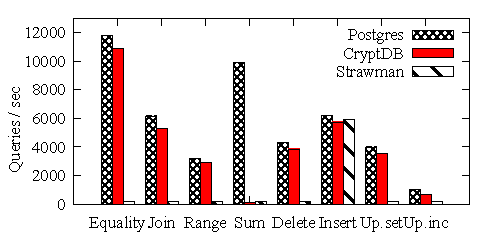
\includegraphics{fig/microbars.pdf} 
\caption{Throughput of the SQL operators from Table~\ref{t:microlat}
  running under \name and Postgres. The numbers on top of the bars
  show the throughput reduction with \name{} for that operator. ``Up. inc" stands for update with increment and ``up. set'' for update set.}
\label{fig:microtput}
\end{figure}


\subsubsection{Storage}

The storage overhead of \name can come from two parts: the proxy
and the DBMS\@.
%The proxy stores only the original schema.
The memory footprint of the \name{} proxy process is
18.5~MBytes in our experiments.
Caching the ciphertext of the 100,000 most common values consumes
$<$1 MByte for $\OPE$ and $\sim$12 MBytes for $\HOM$.  On the DBMS
server, for TPC-C, \name{} increased the database size by 4.5$\times$
due to cryptographic expansion of certain integer fields, all fields being encrypted and most of them being integers. In fact, strings and
binary data remain roughly the same size. Consequently,
for phpBB, \name{} increases server storage by 42\%, caused largely
by the public keys of principals (users, groups and messages) and the
$\HOM$ onion for encrypted integer fields.
As the number of posts in a forum grows, the amortized storage overhead
decreases, because all posts are encrypted for the same forum principal.

% At the DB server, \name increases the size of the database due to
% onion encryption and tables of principal keys.  For TPC-C, the
% database size using Postgres was 135~MB and with \name, it was
% 619~MB, amounting to 4.5 times increase. This is mostly because of
% aggregates which are large cryptographic numbers, without which it is
% a three fold increase.  Since disk space is relatively cheap, we do
% not consider increased storage cost to be a significant barrier to
% adoption of \name.

%Moreover, there is virtually no expansion for large data items such as
%long strings or binaries.  Therefore, a database storing large text
%or binaries (e.g., photos) will have almost no storage overheads.



\begin{figure}[t]
\centering
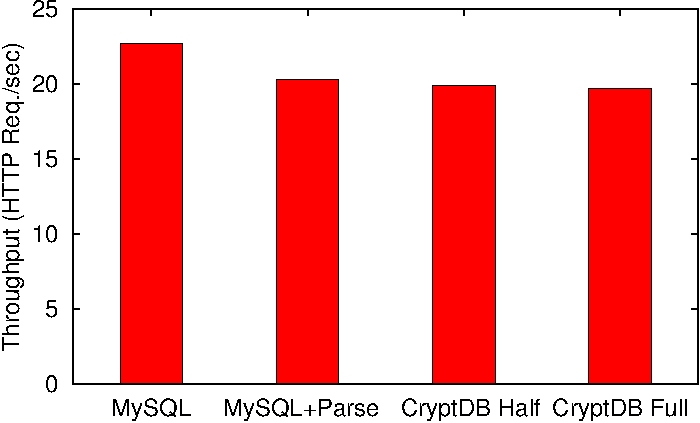
\includegraphics{fig/tputbars.pdf} 
\caption{Throughput comparison for phpBB\@. ``MySQL'' denotes phpBB
running directly on MySQL, ``MySQL+Parse'' includes the parsing cost
of \name{} with cryptography and key management removed, ``\name Half''
shows the whole \name{} with half the annotations, and ``\name{} Full''
is the end-to-end system with all sensitive fields annotated.  Most
HTTP requests involved tens of SQL queries each.  Percentages indicate
throughput reduction relative to MySQL\@.}

\label{fig:appstput}
\end{figure}


% must eval adjustable sec!!





% !TEX root = paper.tex

\section{Related Work}
\label{s:related}

{\bf Search and queries over encrypted data.}
Song et al.~\cite{Dawn-Song-Search-2000} and Amanatidis et
al.~\cite{amanatidis-boldyreva-o'neill} describe cryptographic tools
for searching keywords over encrypted data; we use a hybrid of these
schemes in \name{}.
%Goh~\cite{goh03} and Chang \&
%Mitzenmacher~\cite{Chang04privacypreserving} each develop methods for
%searching over pre-defined encrypted indexes, but applying these
%methods to a DBMS would require substantive changes and would be considerably
%slower than existing index structures.  
Bao et al.~\cite{private-query-multi-user-for-searchable} extend these
encrypted search methods to the multi-user case.
% each user has a different secret key used to encrypt data, but any user can
% search for keywords over all the data.
% and the administrator of the ``semi-trusted'' DBMS server is able to
% revoke privileges. 
%Agrawal et al.'s Hippocratic databases~\cite{hippocratic} address the
%problem of preventing unauthorized users from reading confidential
%data by expressing security policies over data items, but do not
%handle the adversary who gains access to the entire DBMS.
Yang et al. run selections with equality predicates over encrypted
data~\cite{Yang-privacy-preserving-queries}.  Evdokimov and Guenther
present methods for the same selections, as well as Cartesian products
and projections~\cite{encrypt-for-secure-outsource}.  Agrawal et
al. develop a statistical encoding that preserves the order of
numerical data in a column~\cite{agrawal2004order}, but it does not
have sound cryptographic properties, unlike the scheme we
use~\cite{boldyreva-ope}. Boneh and Waters show public-key schemes for
comparisons, subset checks, and conjunctions of such queries over
encrypted data~\cite{queriesEncryptionBoneh}, but these are highly
impractical. 

%Amanatidis et al.~\cite{amanatidis-boldyreva-o'neill} propose methods
%for exact searches that do not require scanning the entire database.

%  \name{} uses ... \hb{what?}  To
% support range queries, this scheme reveals all repeating values and
% all common ranges (same prefix values) in the whole database {\em a
%   priori}, which greatly reduces confidentiality.

% key to our security is the dynamically-adjustable encryption based
% on queries: fields that are never used in range queries or
% equalities should remain encrypted with the strongest encryption
% scheme. Finally, they do not support all other queries besides
% equality and prefix-based ranges, and did not build a system.

%These papers all assume a threat model
%similar to threat 1 from \S\ref{s:model}.  

These techniques are undoubtedly important contributions, but even
with {\em all} of these previous techniques, efficient SQL query
processing is unachievable.  Joins are not supported, order checks are
inefficient, and client-side query processing is required; moreover,
implementing many of these techniques would entail unattractive
changes to the innards of the DBMS, and would require users either to
build and maintain indexes on the data at the server or to perform
sequential scans for every selection/search.  Moreover, none of these
schemes was developed in the context of a prototype system.

%approaches are a good first cut at the problem, but are
%incomplete in substantive ways: none of these support the full set of
%SQL queries, providing mostly only equality comparisons; most require
%significant client-side query processing~\cite{xxx}; and most require
%changing the innards of a DBMS~\cite{xxx}.  In addition, some of these
%proposals are inefficient, for example requiring users either to build
%and maintain indexes on the data at the server or else to perform
%sequential scans for every selection/search.  Finally, none of these
%proposals described a working prototype system.  Nevertheless, these
%approaches are useful for confidential text search, and we use a
%similar method for search queries~\cite{amanatidis-boldyreva-o'neill,
%  Dawn-Song-Search-2000}.



%While early proposals attempted to enable SQL processing over
%encrypted data, their privacy mechanisms were heuristic without formal
%guarantees, required a significant rewrite of the DBMS design, relied
%on considerable client-side processing, and did not support a wide
%range of SQL queries.

Some researchers have developed prototype systems for subsets of SQL,
but they provide no confidentiality guarantees, require a significant
DBMS rewrite, and rely on client-side
processing~\cite{sqlOverEncryption,damianiIndex,Ciriani09keepafew};
one proposal requires trusted entities and two non-colluding
untrusted DBMSs~\cite{two-party-computation}.  Hacigumus et al. split
the domain of possible values for each column into partitions, storing
encrypted data~\cite{sqlOverEncryption}. Each partition has as label a
number and each value in a column is replaced with the number of the
partition.
%By grouping elements in partitions in every column, 
However, confidentiality is often compromised because an adversary can
now learn which elements are close together in value and can see the
order of the partitions.  In addition, clients have to filter query
results.  In contrast, our dynamically-adjustable encryption mechanism
only reveals such relations for those columns that are used in a
filter.
%; as we saw
%in \S\ref{s:eval}, such a mechanism successfully keeps sensitive fields
%encrypted with secure encryptions schemes.  
%Moreover, clients have to perform considerable filtering of query
%results because the server runs the queries on partitions rather than
%actual tuples.  
% Damiani et al.~\cite{damianiIndex} require clients to perform part of
% the query processing, Ciriani et al. require that all sensitive data
% be stored on the clients~\cite{Ciriani09keepafew}, and Chow et
% al.~\cite{two-party-computation} require the presence of two
% non-colluding database systems.
% Ozsoyoglu et
% al.~\cite{Ozsoyoglu03anti-tamperdatabases} use UDFs instead of
% changing DBMS internals, but their approach only applies to integers,
% and does not support joins, updates, or inserts.  More
% problematically, they encrypt fields with a
% \textit{distance}-preserving encryption function for which $a-b = E(a)
% - E(b)$, but this approach provides essentially no confidentiality.

%Such scheme is not secure
%because the mere knowledge of one value $a$ for an encryption $E(a)$
%leaks the decryption of all other encrypted values.

% Some papers have addressed the problem of running queries over XML
% documents or databases~\cite{Wang-xml, querying-encrypted-XML}, but
% suffer from several of the drawbacks mentioned above.  \hb{is that
%   true?  actually these two papers are not real systems.}

%Using these partitions, a server
%tries to process as much of a SQL query as possible, leaving the
%remaining processing for the client.



% provide a solution for processing
% range queries over encrypted data.  Each element in a tuple is
% encrypted and hashed to a small number of buckets to improve
% privacy. Range queries can be computed using a B+ tree, but these are
% done by the trusted client that needs to traverse the B+ tree by
% sequentially performing queries at the server. Such work does not
% support joins, aggregates, or string searches.

% TODO: may want to mention work on splitting values over two dbs, requesting
% multiple queries -- these are heuristics and do not help

% Ciriani et. al~\cite{Ciriani09keepafew} propose a new approach to
% confidentiality: replacing data encryption with fragmentation; they
% store a part of the data at the trusted client (e.g. sensitive columns
% or relations between columns) and the rest of the data unencrypted at
% the untrusted server, thus avoiding encryption altogether. However,
% each client (trusted) has to store a potentially large amount of data
% locally and has to perform query processing whenever sensitive data is
% involved in a query. 
%Moreover, as seen in Section \ref{s:eval}, one
%can use encryption at reasonable overheads.

% Chow et al.~\cite{two-party-computation} require the presence of two
% additional parties, a randomizer and a query engine, which are assumed
% not to communicate; moreover, the data is stored at multiple DBMSs
% that do not trust each other. The security of their protocols hinge on
% such security assumptions and on no collusions happening; such a
% setting is not always possible, and solutions without such strong
% trust assumptions may be desirable.


% At a high level, the main contribution of \name over prior work is a
% practical novel approach to guaranteeing privacy in database-backed
% applications.  To our knowledge, \name is the first private system to
% support all the operators used commonly in SQL, perform virtually all
% the query processing on the server, work without modifying the
% internals of existing relational DBMS codebases or client
% applications, and run at a fairly modest performance degradation.

%Related work to \name{} consists of the following solution approaches.

% us. (2) A large part of the query must be resolved on the client side:
% the client finishes filtering selections and joins, as well as finish
% grouping values. This may require a large amount of data sent to the
% client and considerable client-side processing. In \name, queries
% are completely evaluated on server side. (3) Such solution does not
% support some functionality like aggregates and search on strings.  (4)
% Importantly, the design of such a database changes radically the
% design of current databases that have been heavily optimized. (5) Such
% a database system has not been built to prove its practicality.

% \vspace{-0.2cm}

{\bf Untrusted servers.}
SUNDR~\cite{li:sundr} uses cryptography to provide privacy and
integrity in a file system on top of an untrusted file server.  Using
a SUNDR-like system, SPORC~\cite{feldman:sporc} and
Depot~\cite{mahajan:depot} show how to build low-latency applications,
running mostly on the clients, without having to trust a server.
However, existing server-side applications that involve separate
database/storage and application servers cannot be used with these
systems unless they are rewritten into distributed client-side
applications to work with SPORC or Depot; moreover, many applications
are not amenable to such a structure.
In contrast, \name{} provides cryptographic privacy guarantees to
existing database-backed applications.
%On the other hand, because \name{} allows the application server to
%perform any computation, it provides no confidentiality guarantees
%under threat 2 of \S\ref{s:model} for users who were logged in at the
%time of a compromise.

%reveals plaintext data to the
%server for any principals that are currently accessing the
%application, so that the server can perform arbitrary computations on
%the data.


{\bf Software security.}  Many tools help programmers either find or
mitigate mistakes in their code that may lead to vulnerabilities,
including static analysis tools like PQL~\cite{livshits:javasec, martin:pql} and
UrFlow~\cite{chlipala:urflow}, and runtime tools like
Resin~\cite{yip:resin}.
%These tools prevent an adversary
%from exploiting certain types of vulnerabilities by assuming that
%certain components of the system are uncompromised, 
In contrast, \name{} provides privacy guarantees for user data
\textit{even if the adversary gains complete control over the
  application and database servers}.  These tools provide no
guarantees in the face of this threat, but in contrast, \name cannot
provide privacy in the face of vulnerabilities that trick the user's
client machine into issuing unwanted requests (such as cross-site
scripting or cross-site request forgery vulnerabilities in web
applications).  As a result, we anticipate using \name{} together with
these tools to improve overall application security.

Rizvi et al.~\cite{rizvi:fine-grained} and
Chlipala~\cite{chlipala:urflow} specify (and enforce) an application's
security policy over SQL views.  \name{}'s SQL annotations can capture
most of these policies, except for result processing being done in the
policy's view, such as allowing a user to view only aggregates of
certain data.  Unlike prior systems, \name{} enforces SQL-level
policies cryptographically, without relying on compile-time or
run-time permission checks.

% There has been work on designing tools for searching on encrypted data
% and work proposing search on encrypted data for outsourcing DBMS
% privately~\cite{Dawn-Song-Search-2000, Chang04privacypreserving,
%   queriesEncryptionBoneh, private-query-multi-user-for-searchable,
%   amanatidis-boldyreva-o'neill, Yang-privacy-preserving-queries,
%   encrypt-for-secure-outsource}. 
% The work in~\cite{private-query-multi-user-for-searchable} also considers the
% multi-user case.


% recognized that, for a
%privacy-preserving DBMS to be practical at all, one should be willing to reveal
%access patterns needed for the desired class of computation.  They also
%stressed the importance of formally specifying and proving the security
%guarantees of a system to prevent attacks, as we proceed in \name{}.  Their
%work is a cryptographic protocol that allows equality comparisons in a similar
%way to $\DET$ and some limited ranges.

% Amanatidis et al.~\cite{amanatidis-boldyreva-o'neill}, propose encrypting all data with a scheme allowing range queries like OPE: revealing {\em a priori} all repeating values and all common ranges
% (same prefix values) in the whole database (across all columns and rows). This approach leaks significant confidentiality; key to our security is the
% dynamically-adjustable encryption based on queries: fields that are never used
% in range queries or equalities should remain encrypted with the strongest
% encryption scheme. Finally, they do not support all other queries besides
% equality and prefix-based ranges, and did not build a system.

% In addition, the privacy provided by the most secure of these
% previously developed schemes is approximately similar to \name.  For
% example, in Yang et al.'s work~\cite{Yang-privacy-preserving-queries},
% after one query has been made, the server only knows the repetitions
% of the constant in the selection filter, and does not know all the
% repetitions of data in a column as in \name.  Therefore, after one
% equality query, their protocol is more secure. However, after a few
% different queries with the same structure, but different constants,
% \name reveals as much information as their approach. These are
% specific tools and do not enable to server to perform other
% requirements in a DBMS: general range queries, updates of a whole
% column or range of tuples (e.g. increments), aggregates, some cannot
% support joins.

% There is also work allowing the server to build secure
% indexes~\cite{goh03} on encrypted data without having access to the
% data. These approaches require significant changes to the DBMS and would not be
% as portable. Moreover, due to complex cryptographic tools they are
% slower. In our case, the server builds indexes naturally as it would
% on typical (longer) numbers. Ge and Zdonik~\cite{c-store-index} enable
% comparisons and designs indexes for a column store.

%There has been work on processing queries on encrypted
%XML. This work provides useful
%security semantics for XML data, but requires a cumbersome DBMS
%rewrite.
% When applying it to the general
%setting of outsourced databases, there are the following issues: they
%change query processing at the server and requires a rewrite of the
%DBMS\@. 
%Moreover, the results sent to the client are a superset of the true
%result, requiring the client to perform additional post-processing.
%which can sometimes be time consuming and bandwidth wasteful. 
%They also do not discuss updates and inserts.
%, and some are in fact
%search on encrypted data and suffer from similar issues as above when
%applying in our context.

% \paragraph{Theoretical approaches.}
% Theoretical solutions, such as recent work based on fully homomorphic
% encryption~\cite{gentryVerifiable} enables an untrusted party to
% perform any general computation on encrypted data without leaking even
% access patterns to the data. Unfortunately, such approach is
% prohibitively impractical; for example, an author of these schemes
% estimates that a simple string search using fully homomorphic
% encryption is about a trillion times slower than without
% encryption~\cite{trillion}.

% Work in PIR~\cite{pir-survey} allows a user to request a tuple from the database
% without the server learning what tuple was requested. While they provide
% excellent security, such approaches are highly infeasible because, for each
%tuple requested, the server must scan the whole database.
 
{\bf Privacy-preserving aggregates.}
Privacy-preserving data integration, mining, and aggregation
schemes (e.g.~\cite{Kantarcioglu-Clifton-2005, Xiong-2007}) are
useful, but not usable by many applications because they only support
specialized query types and require a rewrite of the DBMS\@.
Differential privacy~\cite{dwork-survey} is complementary
to \name{}; it allows a trusted server to decide what answers to
release and how to obfuscate answers to aggregation queries to avoid
leaking information about any specific record in the database.
% Differential privacy has a different,
%complementary goal from \name{}.
%, but it could be used in concert with \name{}: \name's proxy
%can decide using these tools when and how to release the answer to a
%query.

% and model from \name; in
% fact, one can add differential privacy to the front end in \name tot
% provide to users only privacy-preserving answers.

%% computing over encrypted data

% Maybe mention attribute-based encryption, where Waters et al. use
% algebraic structure of encrypted data to extract statistics.

{\bf Query integrity.}
%Although \name{} does not provide integrity for query results in the
%face of a compromised database server, 
Techniques to ensure integrity for SQL queries can be integrated into
\name{} because \name{} allows relational queries on encrypted data
to be processed just like on plaintext.
%most proposed approaches can be incorporated readily into \name{},
These methods can provide integrity by adding a MAC to each
tuple~\cite{li:sundr,plutus,sirius}, freshness using Merkle or chained
hashes~\cite{plutus,cloudproof,sirius}, and both freshness and
completeness of query results using the approach
in~\cite{queryassurance}.  
%Also, Thompson et al.
In addition, the client can verify the results of aggregation
queries~\cite{Thompson_privacy-preservingcomputation}, and provide
query assurance for most read queries~\cite{sion-assurance}.


%A malicious server can
%affect three aspects of data security: integrity, freshness, and
%completeness. Integrity is solved by adding a MAC to each tuple as
%in~\cite{li:sundr,plutus,sirius}. Freshness has been addressed using
%Merkle hashes or chained hashes~\cite{plutus,cloudproof,sirius} and
%both freshness and completeness of query results are addressed
%in~\cite{queryassurance}.

\nz{Navajo Systems~\cite{navajo}.}


\section{Conclusion}
\label{s:concl}

We presented \name{}, a system that provides practical and provable
confidentiality in the face of two significant threats---curious DBAs
and arbitrary compromises of the application server and
DBMS---confronting database-backed applications.  \name{} meets its
goals using three ideas: running queries efficiently over encrypted
data using a novel SQL-aware encryption strategy, dynamically
adjusting the encryption level using onions of encryption to minimize
the information revealed to the untrusted DBMS server, and chaining
encryption keys to user passwords in a way that allows only authorized
users to gain access to the same encrypted data.  The developer effort
required to express confidentiality policies for multi-user
applications is small, ranging between 11 and 13 unique annotations of
the application's database schema across three existing applications
(phpBB, HotCRP, and grad-apply).  The throughput penalty of \name{} is
modest, about \tput{} for the TPC-C benchmark and 13\% for our
synthetic phpBB workload.  Our results suggest that \name{} is useful
for applications where the ability to run confidentially over an
untrusted or outsourced infrastructure trumps achieving the highest
possible performance.

The source code for CryptDB is available for download at
\url{http://css.csail.mit.edu/cryptdb/}.

% This paper presented \name, a practical and novel system for ensuring
% data privacy on an untrusted SQL DBMS server.  \name uses three novel
% ideas to achieve its goal: an {\em SQL-aware encryption strategy},
% {\em adjustable query-based encryption}, and {\em onion encryption}.
% As part of \name's SQL-aware encryption strategy, we propose
% optimizations for existing cryptographic techniques, as well as a new
% cryptographic mechanism for private joins.  Our prototype of \name
% requires no changes to application or DBMS server code, and uses
% user-defined functions to perform cryptographic operations inside an
% existing DBMS engine, including both Postgres and MySQL\@.  Under a
% TPC-C workload, our prototype incurs a \tput reduction in throughput
% compared to an unencrypted DBMS, making \name a practical option for
% privacy-sensitive data.


\section*{Acknowledgments}

The authors would like to thank Carlo Curino, Craig Harris, Frans
Kaashoek, Sam Madden, the anonymous reviewers, and our shepherd, Adrian
Perrig, for their helpful feedback.  Carlo Curino and Evan Jones provided
traces used in our TPC-C evaluation. Eugene Wu and Alvin Cheung also
provided useful advice. This work was supported by the NSF (CNS-0716273
and IIS-1065219) and by Google.



{
\small
\setlength{\bibsep}{3pt}
\bibliographystyle{abbrv}
\bibliography{n-str,cryptdb,n,n-conf}
}



\end{document}
